\chapter{Diversité} \label{ch:DIV}

\section{Mesures et méthodologie}

L'objectif du travail est de quantifier l'impacte de la diversité sur la propagation de pandémies. Cette section est dédié à la prises de mesures avec des niveaux de diversité différents et d'en constater les résultats. Afin de ne pas trop complexifier le modèle au delà des simulations SIR, nous ne modifions que le paramètre de diversité ainsi que la charge virale. D'autres paramètres du modèle pourraient être étudié mais ce chapitre ne les explore pas.\\

Toutes les musures de diversité ont été effectuées sur des systèmes aux paramètres semblables. La taille des systèmes est définie à $1264\times 1264$ avec une population de $10^5$ individus, il s'agit de systèmes en densité $\frac{1}{16}$. Un exemple de fichier de configuration est donné ci-dessous.

\begin{minted}
	[
	frame=lines,
	framesep=2mm,
	baselinestretch=1.2,
	bgcolor=LightGray,
	fontsize=\footnotesize,
	linenos
	]
	{c++}
	
	TAILLE_SYSTEME = 1264
	NOMBRE_INDIVIDUS = 100000
	ITERATIONS = 5000
	RERUN_LIMIT = 100
	FAIL_SEUIL = 30
	GENOME_INIT_I = 0
	GENOME_DIVERSITY_I = 8
	GENOME_INIT_AP = 0
	VITESSE_MUTATIONS_AP = 0
	CHARGE_VIRALE = 1
	PARAMETRE_FONCTION = 4
	CELLULE_AP = 0
	SURVIE_AP = 0
	NOMBRE_MOUVEMENT = 1
	PERFECT_MIX = true
	TEMPS_AVANT_IMMUNITE = 1
	IMMUNITE_MECANISME = true
	RESISTANCE_MECANISME = false
\end{minted}

L'exemple de fichier de configuration produit une simulation au mélange parfait avec une diversité de $8$. La configuration est similaire à celle d'une simulation SIR, la seule différence ici est l'ajout d'un paramètre de diversité non égal à $0$.\\

Toutes les simulations qui suivent se basent sur ce fichier de configuration mais avec quelques modifications.\\

Premièrement, le niveau de diversité varie d'une simulation à une autre. Les valeurs de diversité choisie sont : $4,8,16,32$. Pour rappel, une diversité de $x$ signifie que $x$ bits des génomes des individus seront complémentés et ceci alétoirement. Sans diversité les génomes des individus sont tous identiques.\\

Deuxièmement, le mode de mouvement ainsi que le nombre de mouvements varie. Seule la première simulation servant d'exemple utilise le mode de mouvement au mélange parfait, toutes les autres ont un nombre de mouvements défini. Les mouvements étudiés sont : $1,10,50$.\\

Finalement nous faisons varier le paramètre de charge virale (ici défini à 1). L'idée principale est ralentir la propagation de pandémies en diminuant la contagion des agents pathogènes. Les simulations sont effectuée sur $4$ niveaux de charge virale : $0.25,0.5,0.75,1$\\

Les résultats du chapitre se découpent en $5$ parties. La première sert d'exemple et permet d'expliquer les mécaniques derrière la diversité. Les $4$ autres parties explorent les $4$ niveaux de mouvements, les $4$ niveaux de diversité et les $4$ niveaux de charge virale.

\section{Résultats}



\begin{figure}[h]
	\centering
	\captionsetup{justification=centering}
	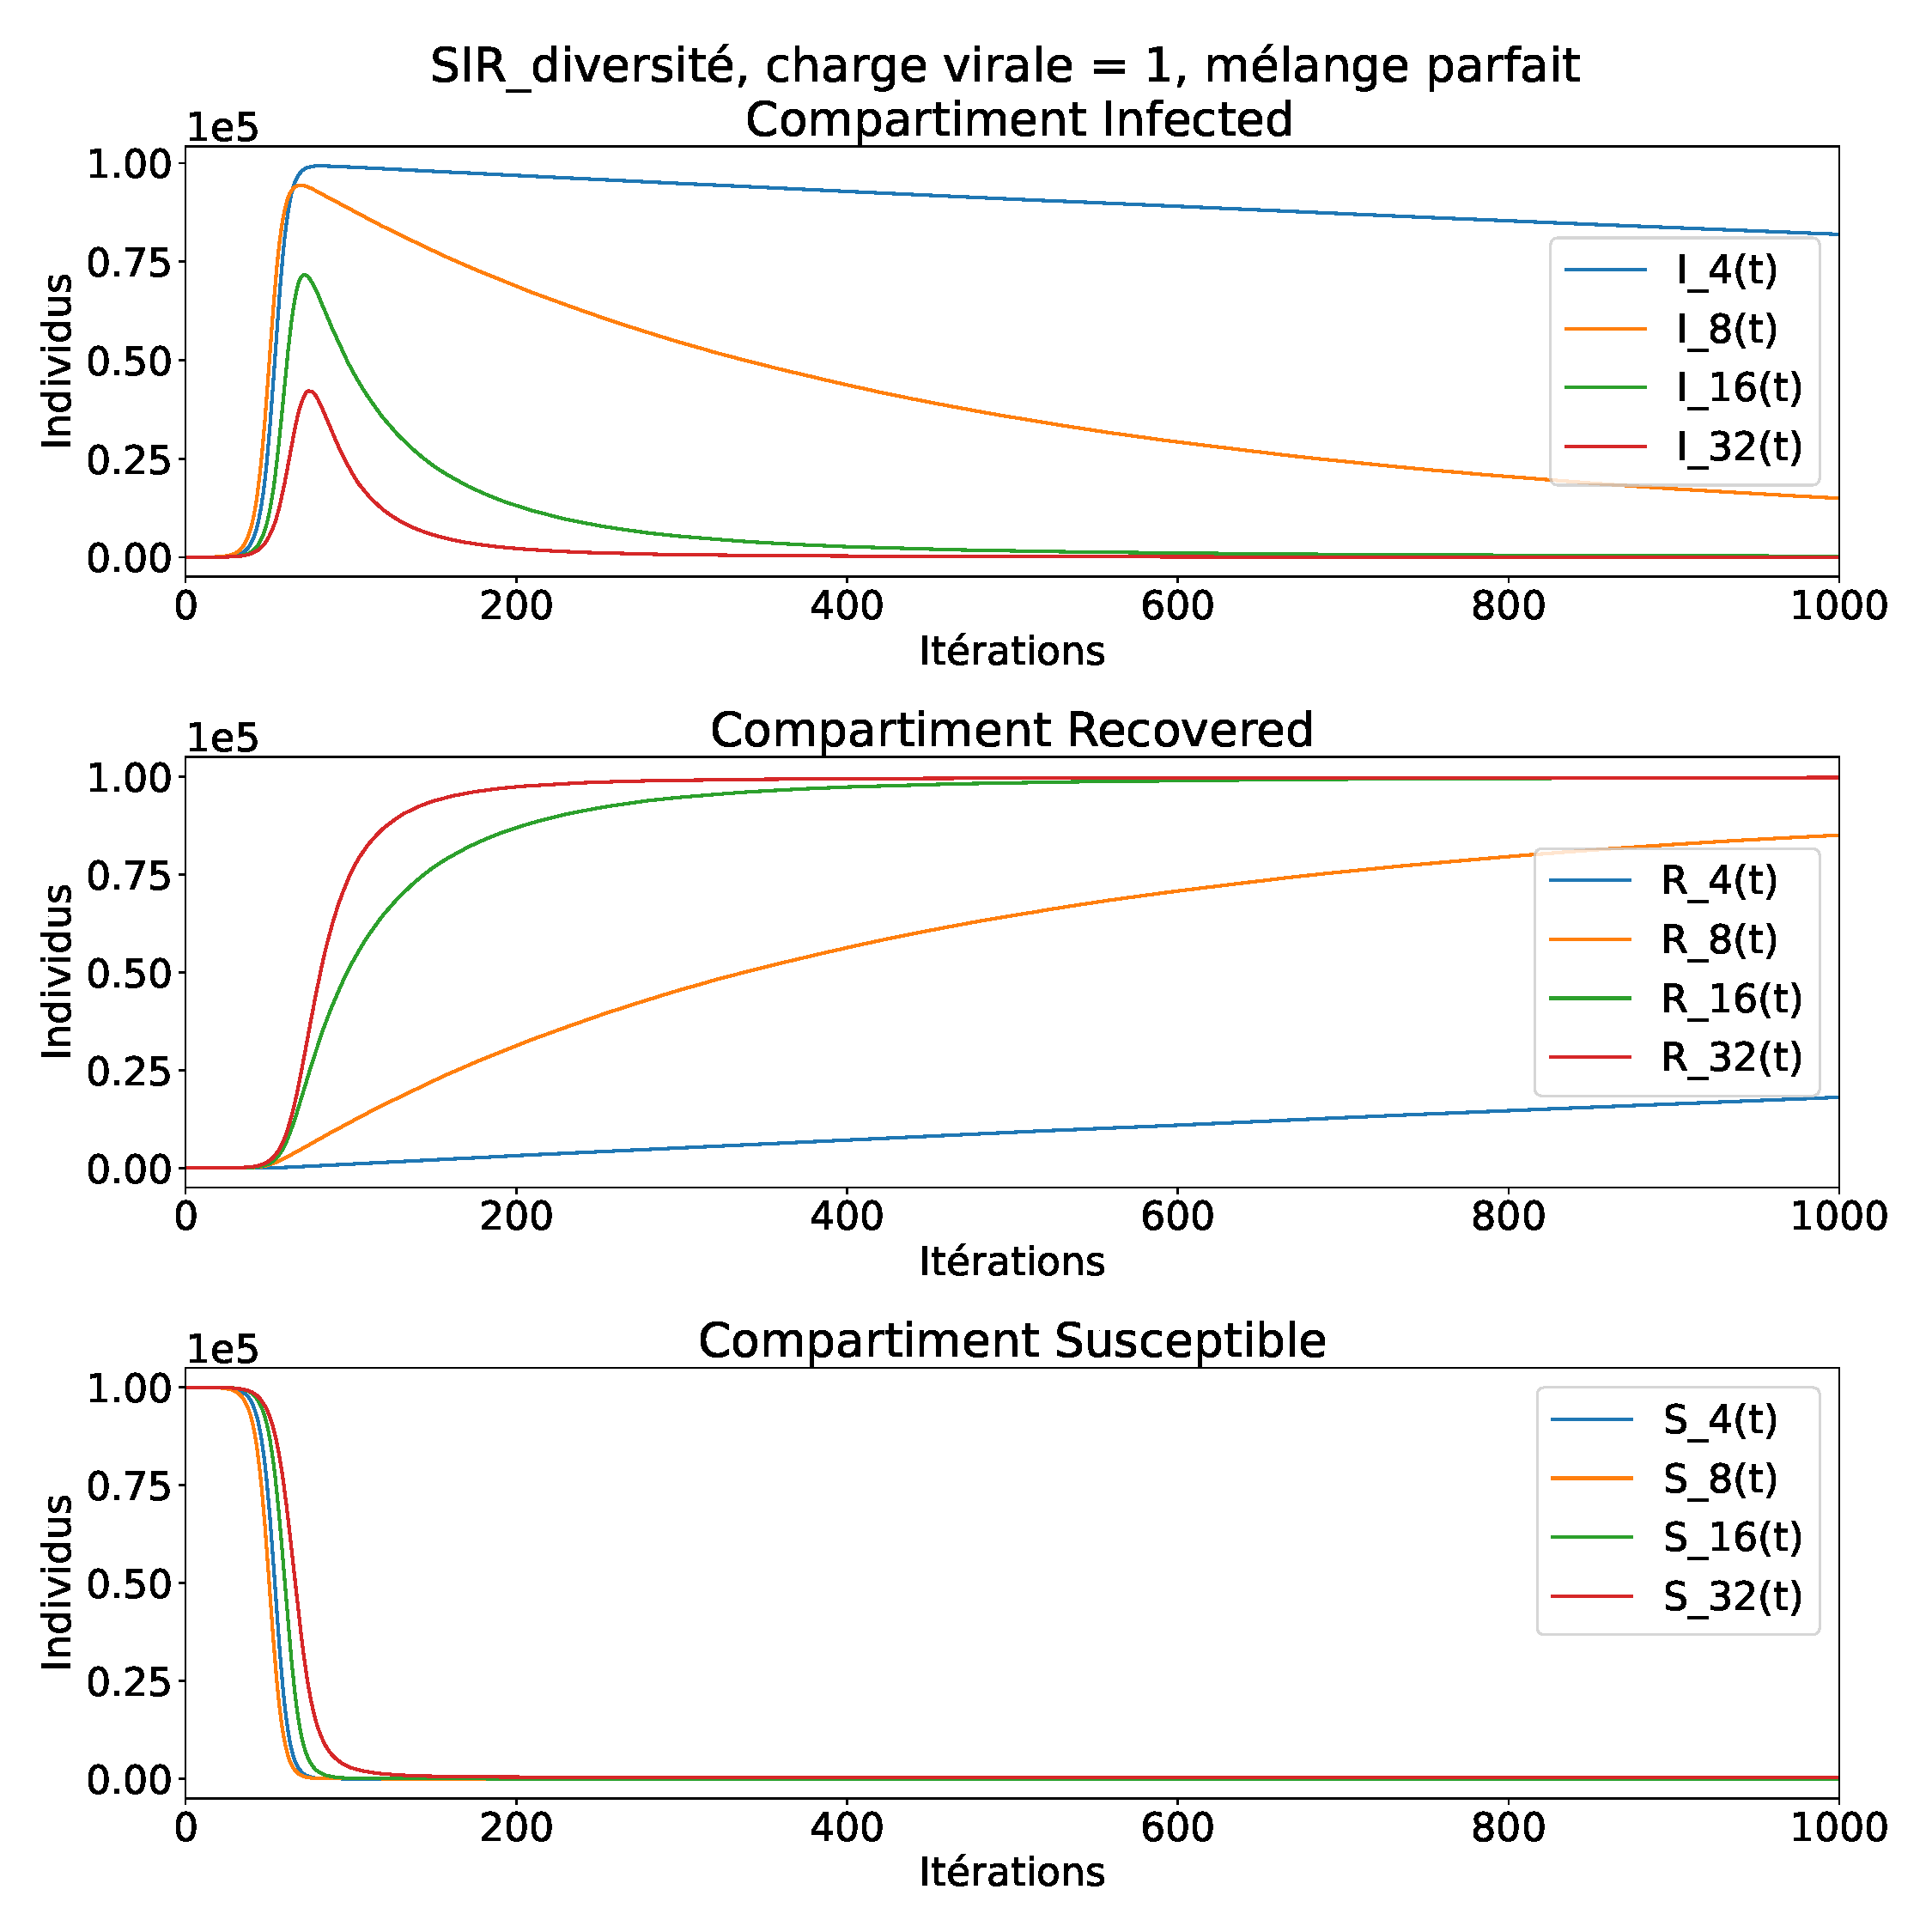
\includegraphics[width=.7\textwidth]{Images/SIR_diversite_mix.pdf}
\end{figure}

\newpage

\begin{figure}[h]
	\centering
	\captionsetup{justification=centering}
	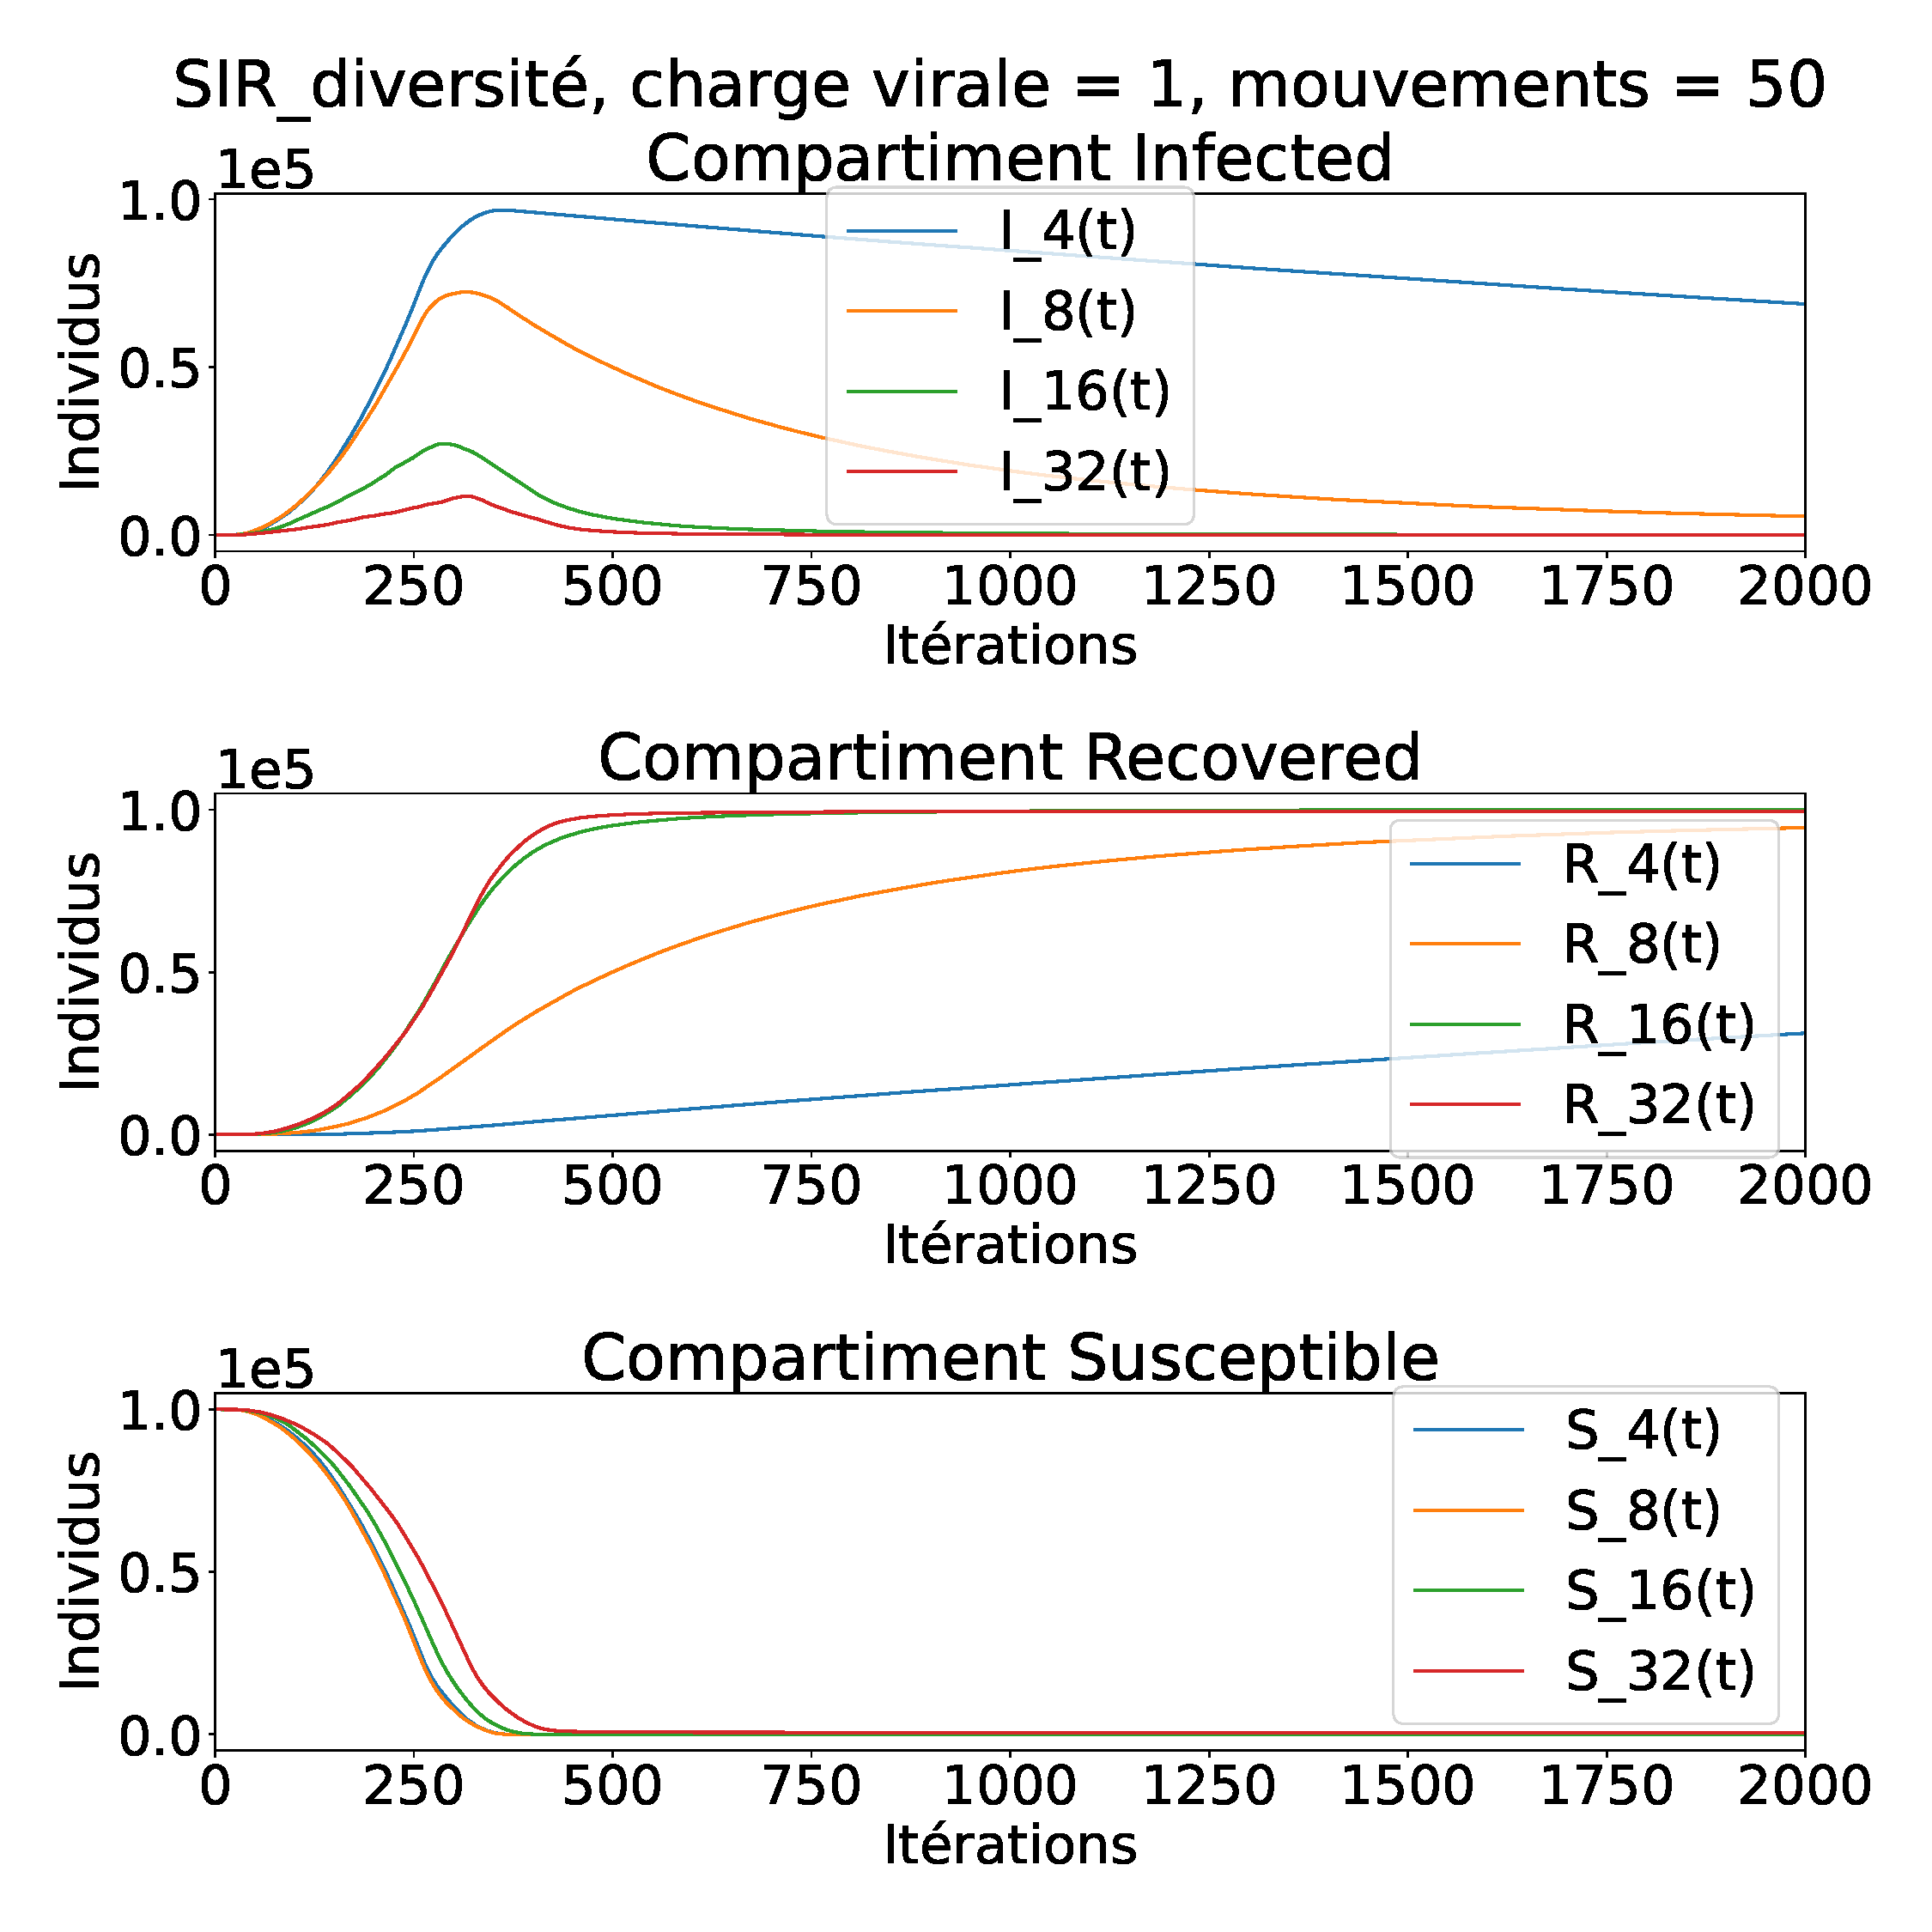
\includegraphics[width=.4\textwidth]{Images/SIR_diversite_1_50.pdf}
	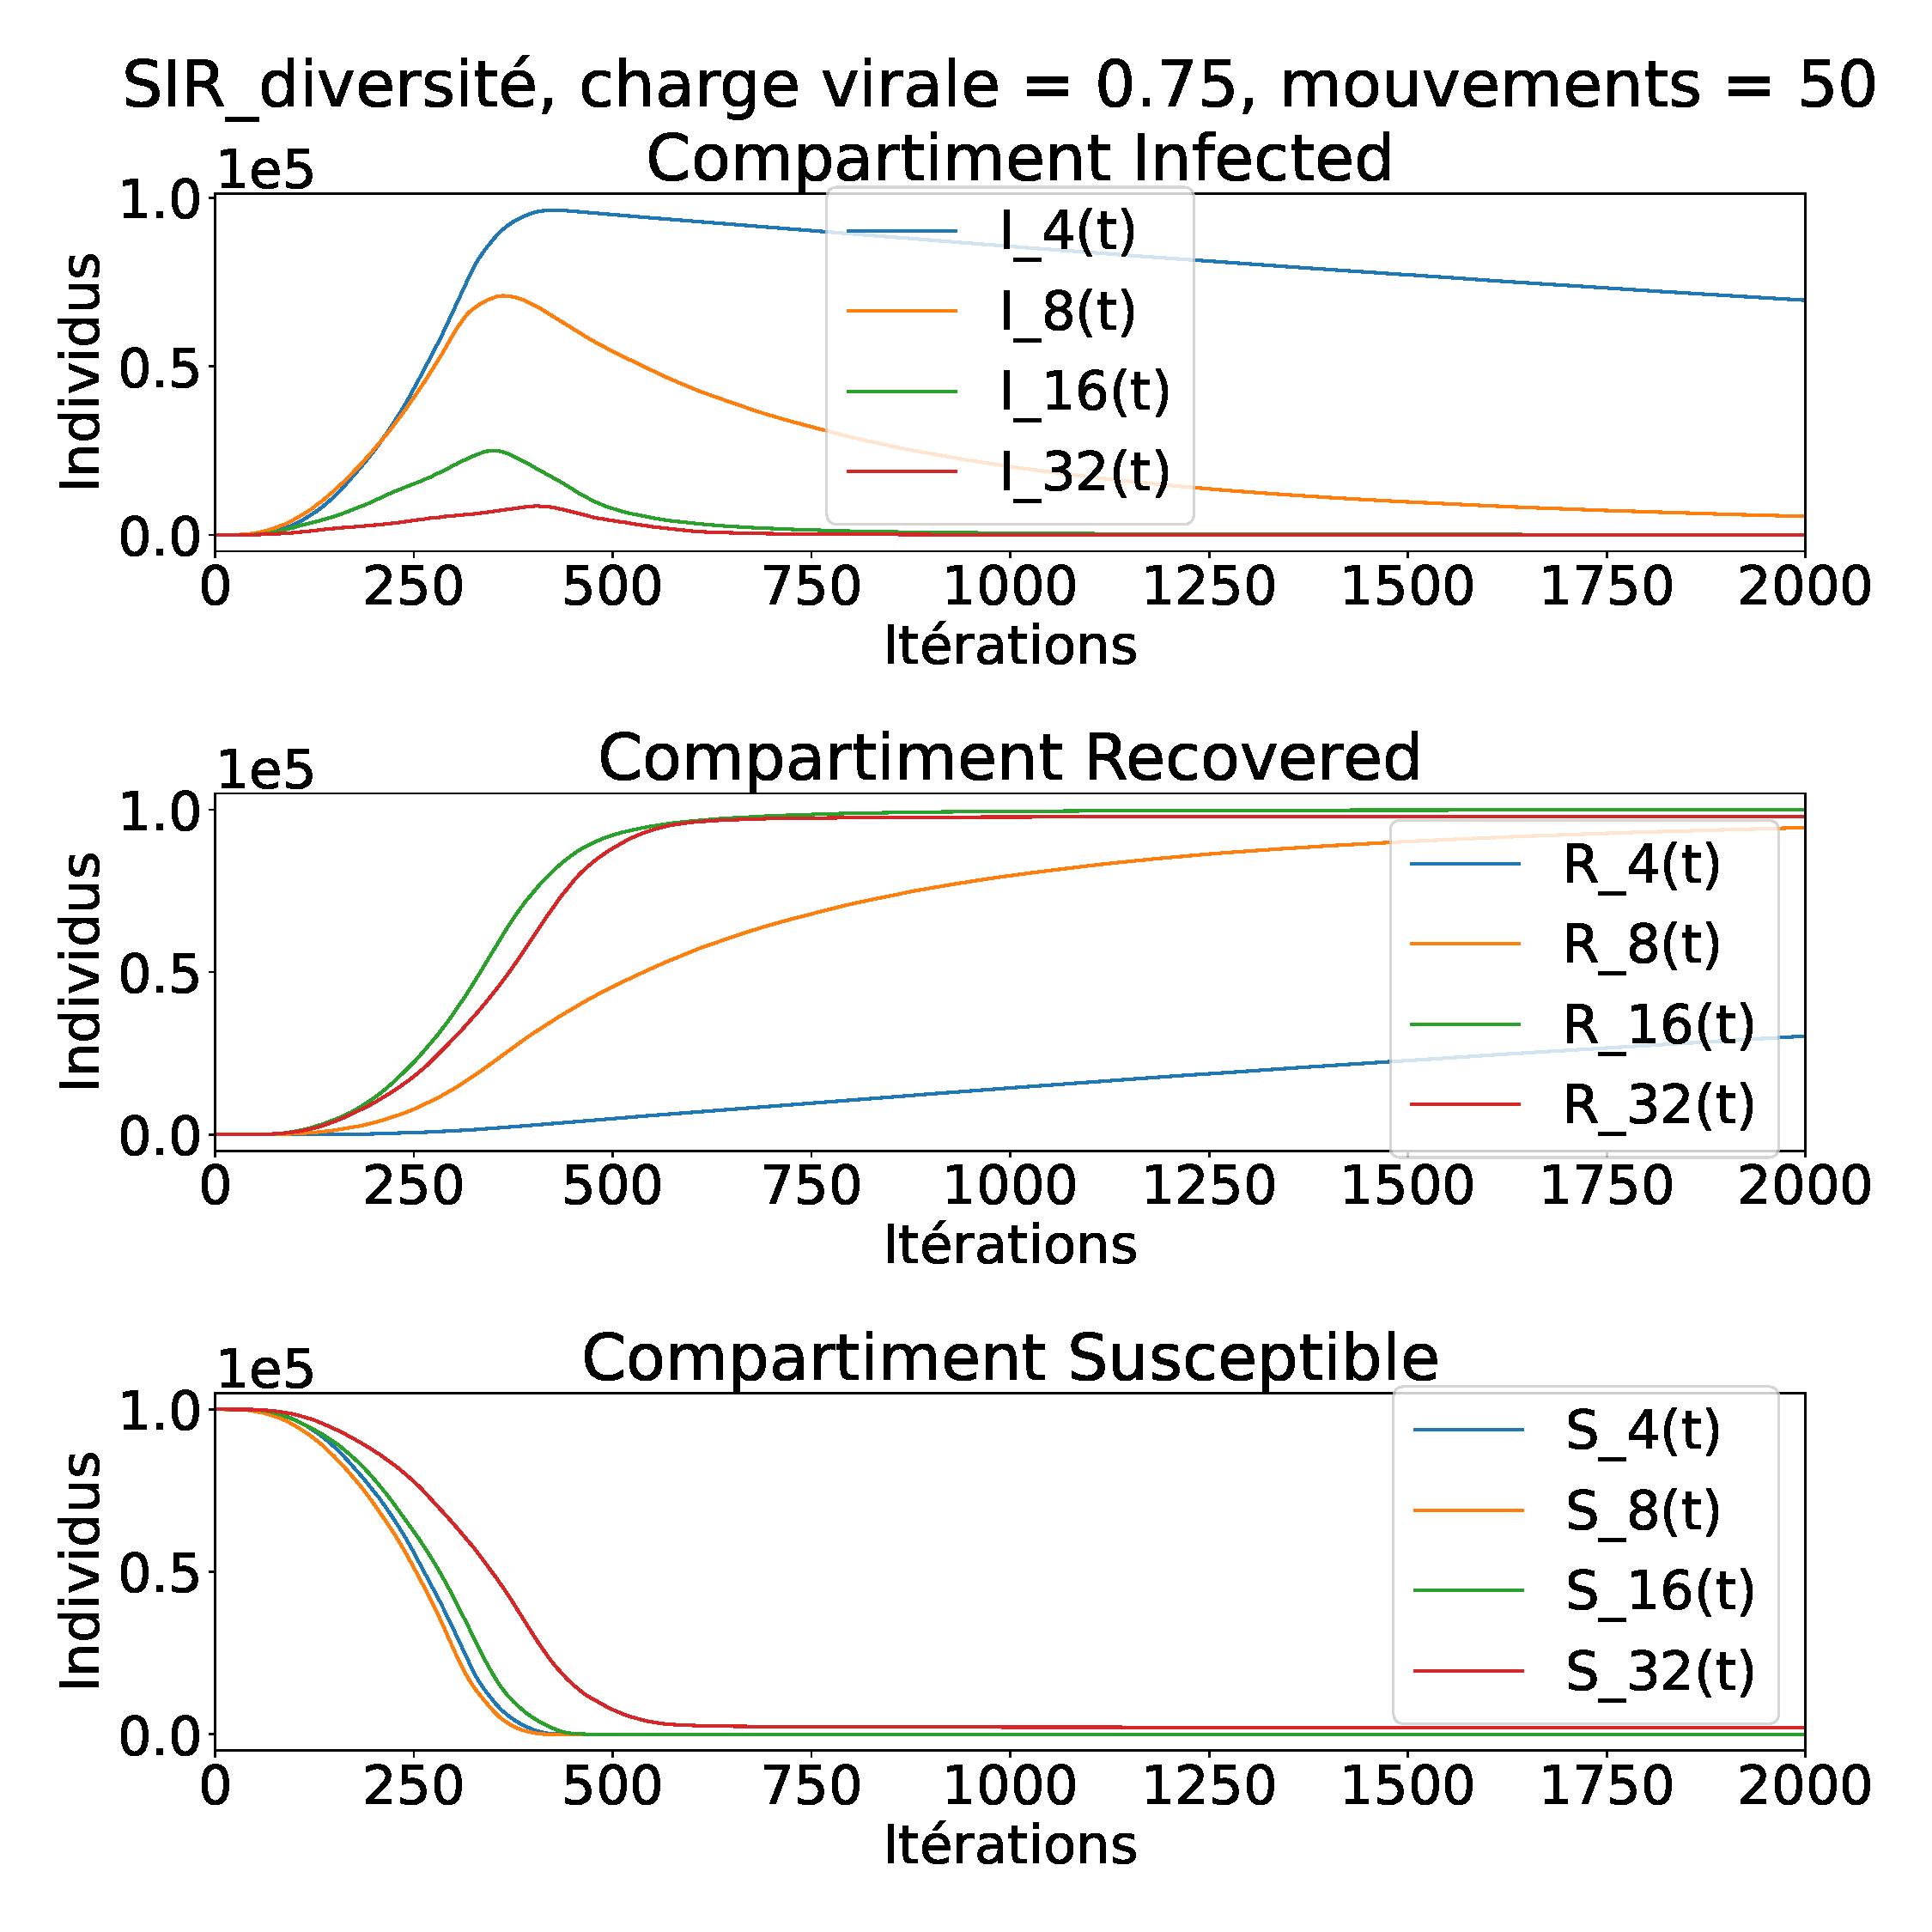
\includegraphics[width=.4\textwidth]{Images/SIR_diversite_075_50.pdf}
	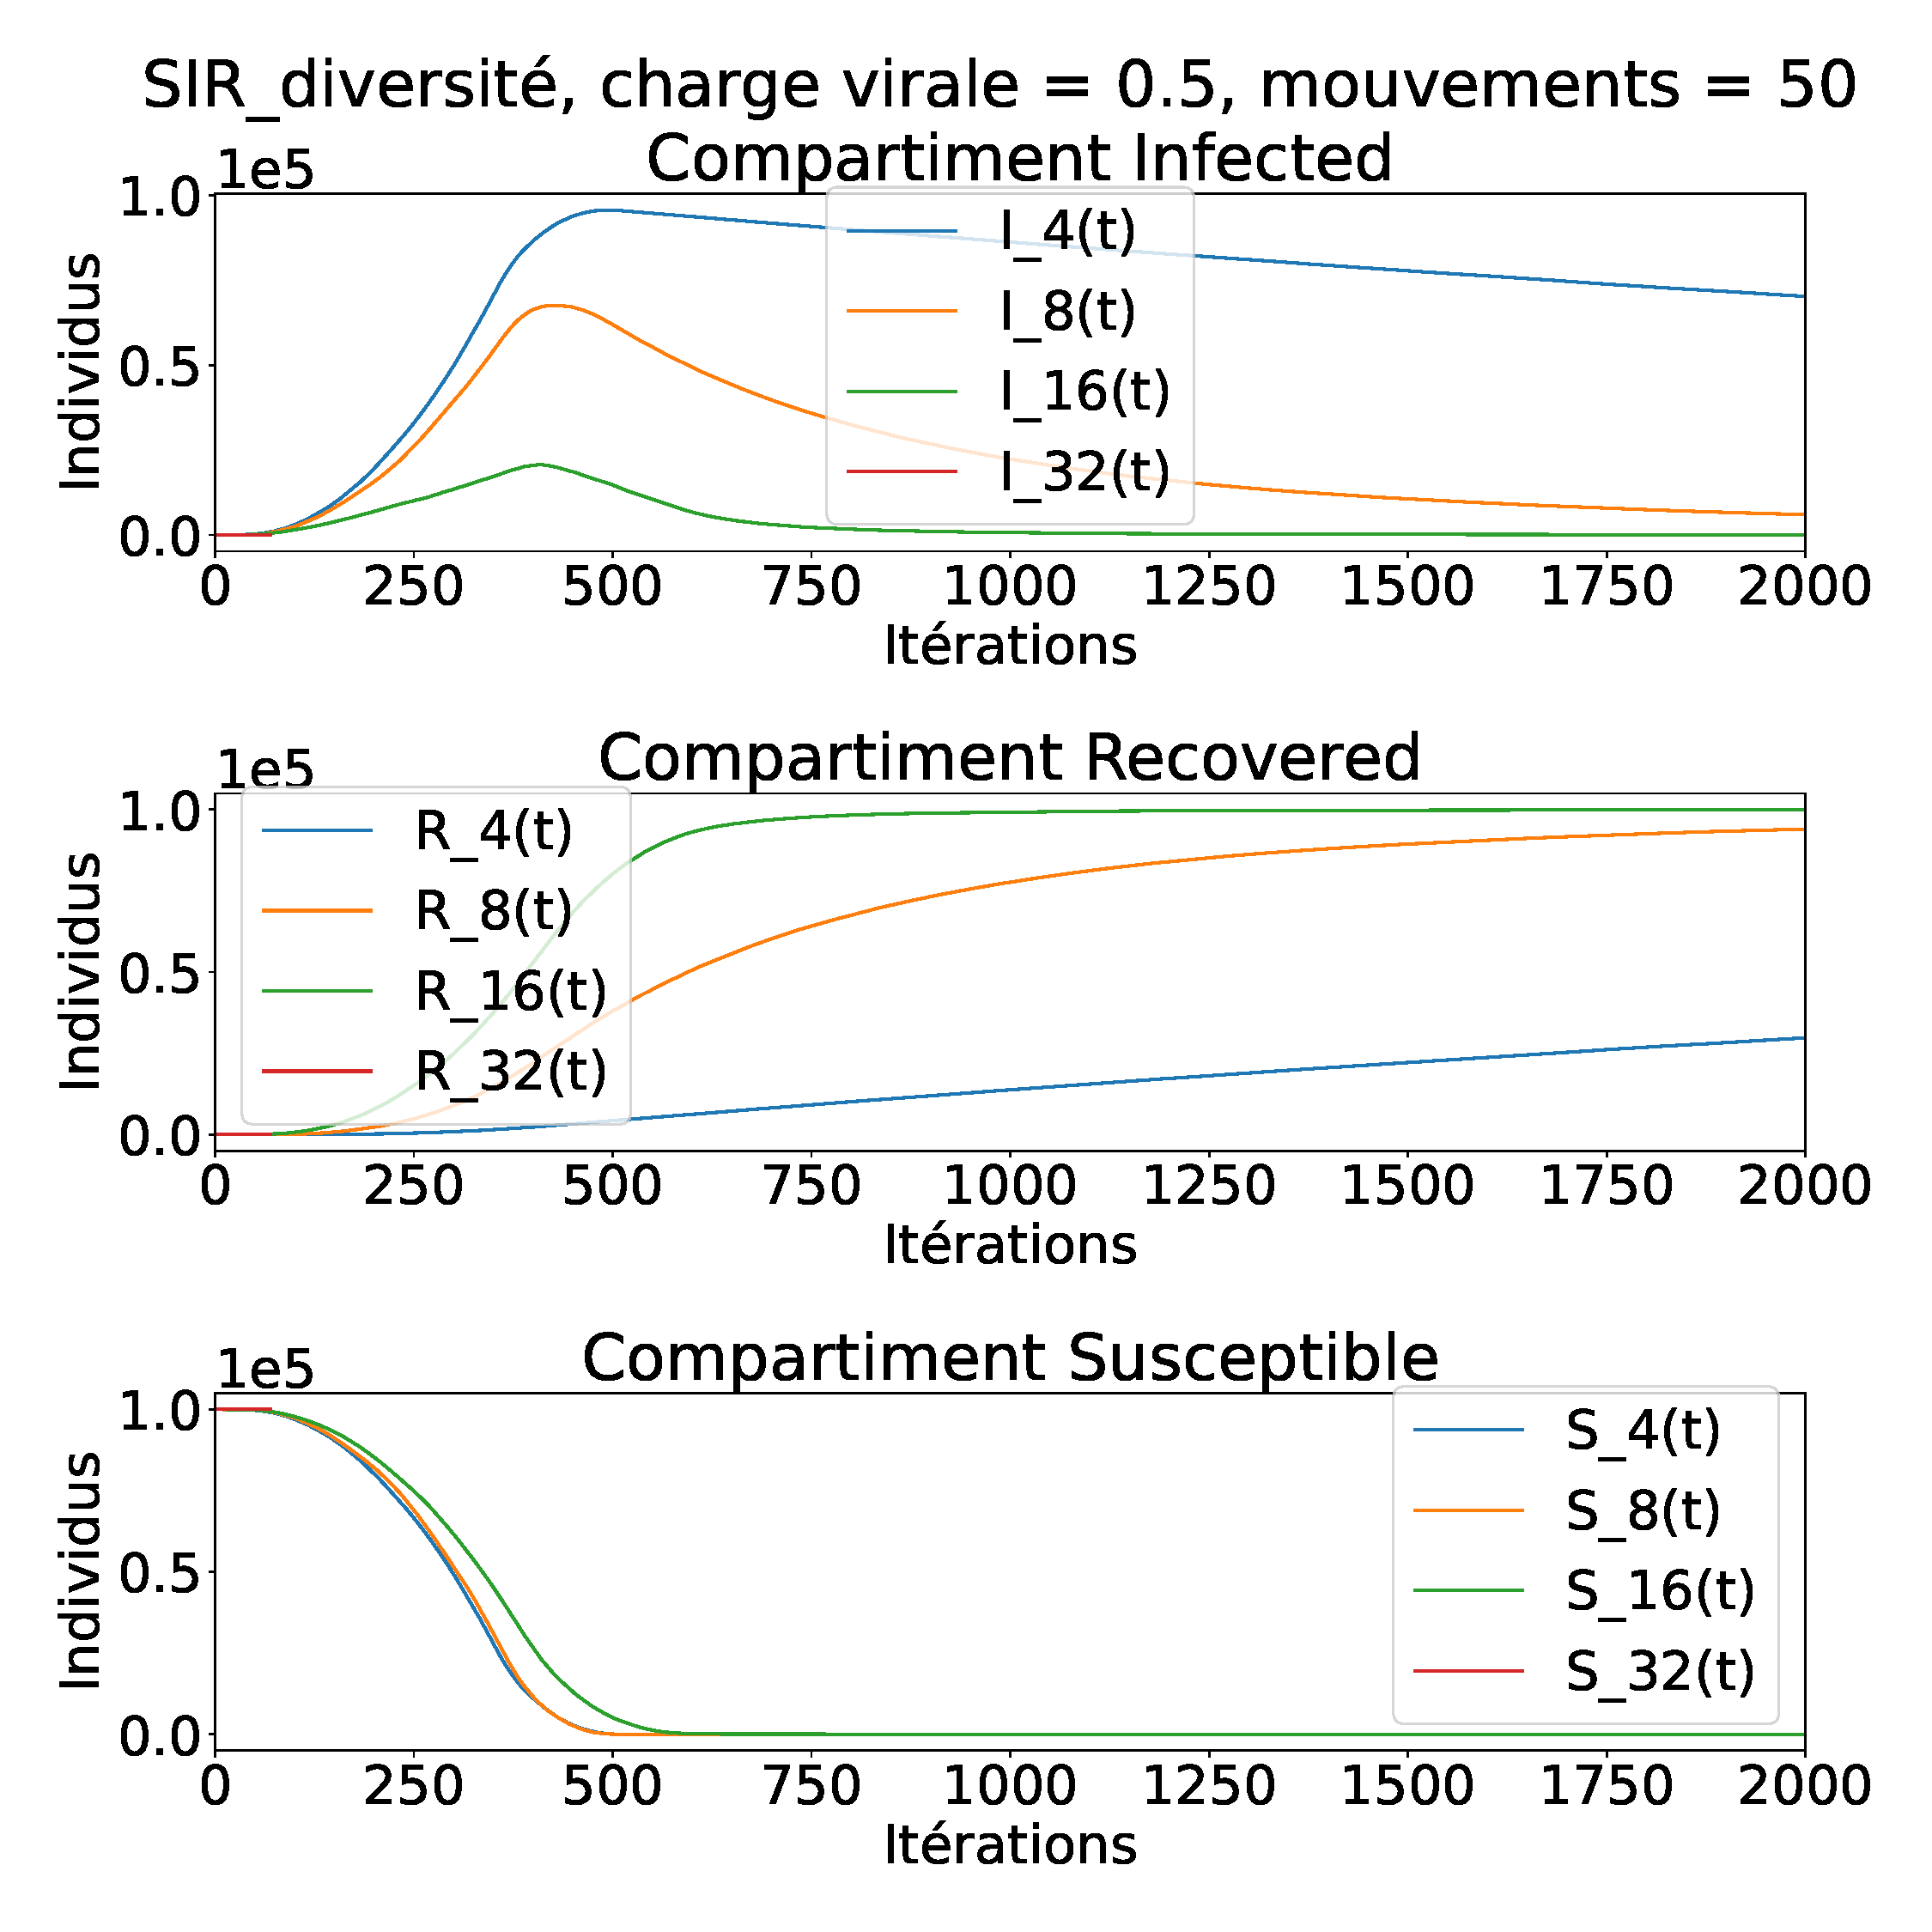
\includegraphics[width=.4\textwidth]{Images/SIR_diversite_05_50.pdf}
	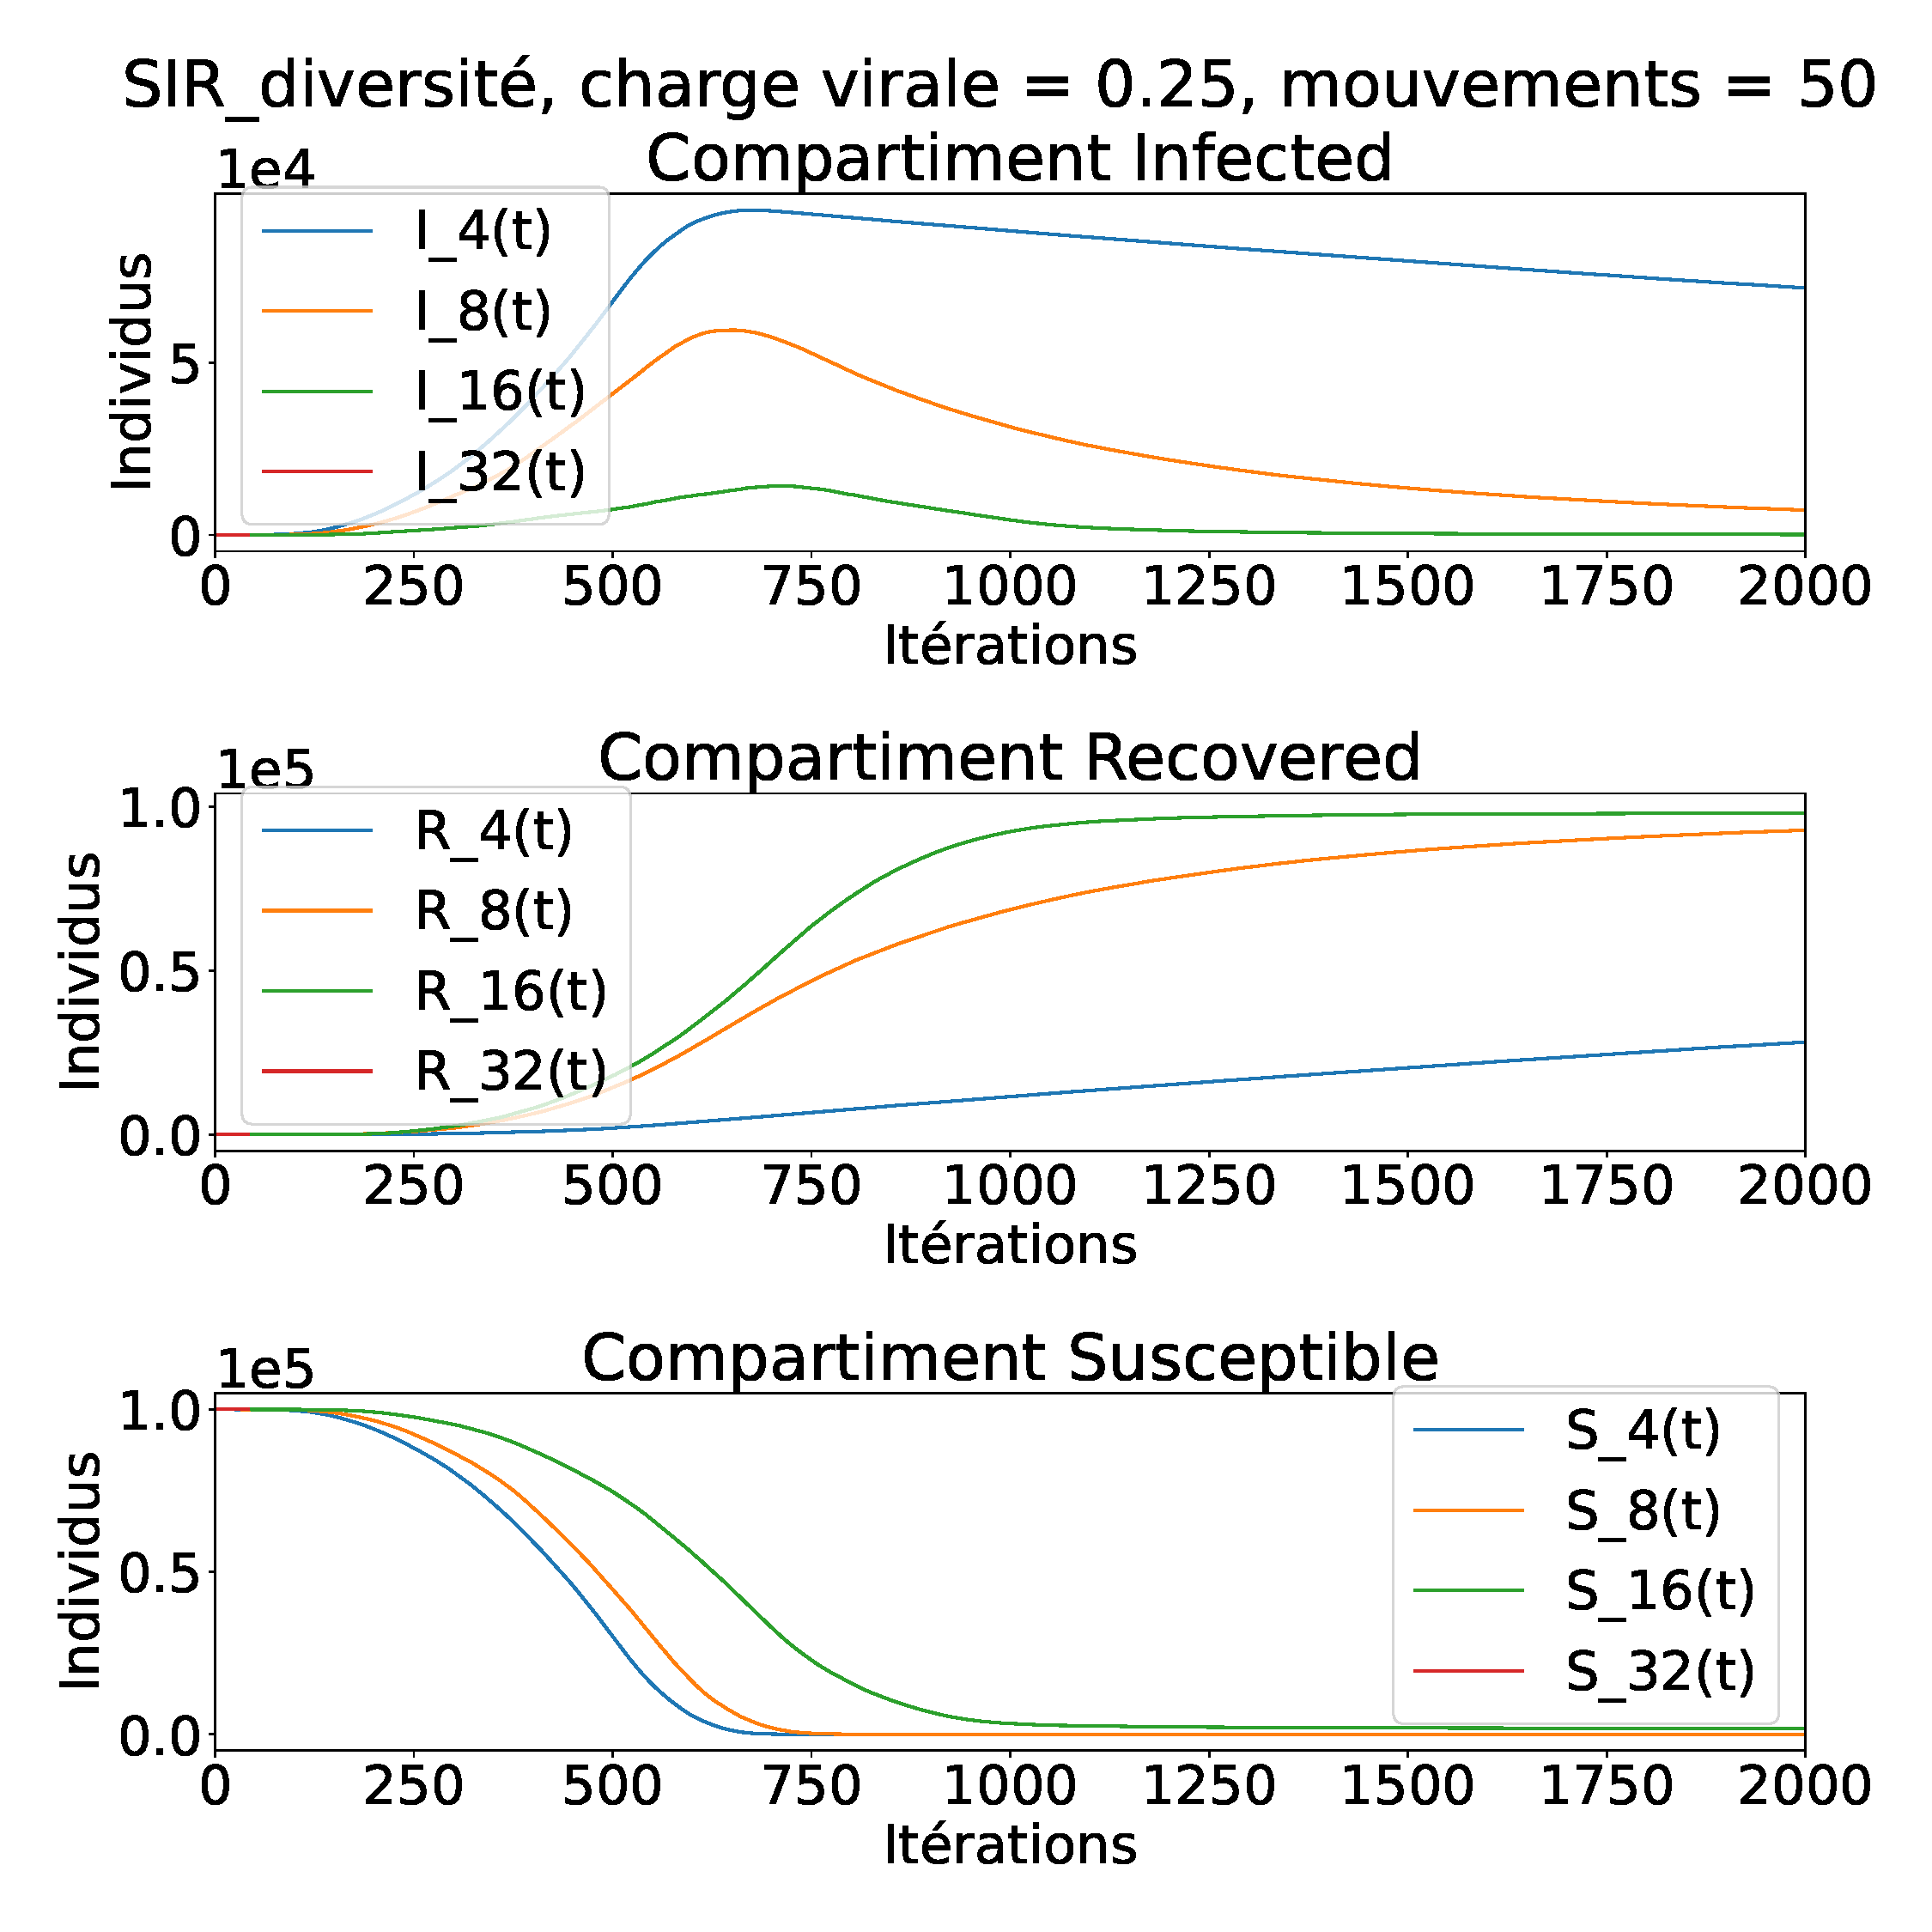
\includegraphics[width=.4\textwidth]{Images/SIR_diversite_025_50.pdf}
	\caption{Comparaison 50 mouvements}
\end{figure}

\newpage

\begin{figure}[h]
	\centering
	\captionsetup{justification=centering}
	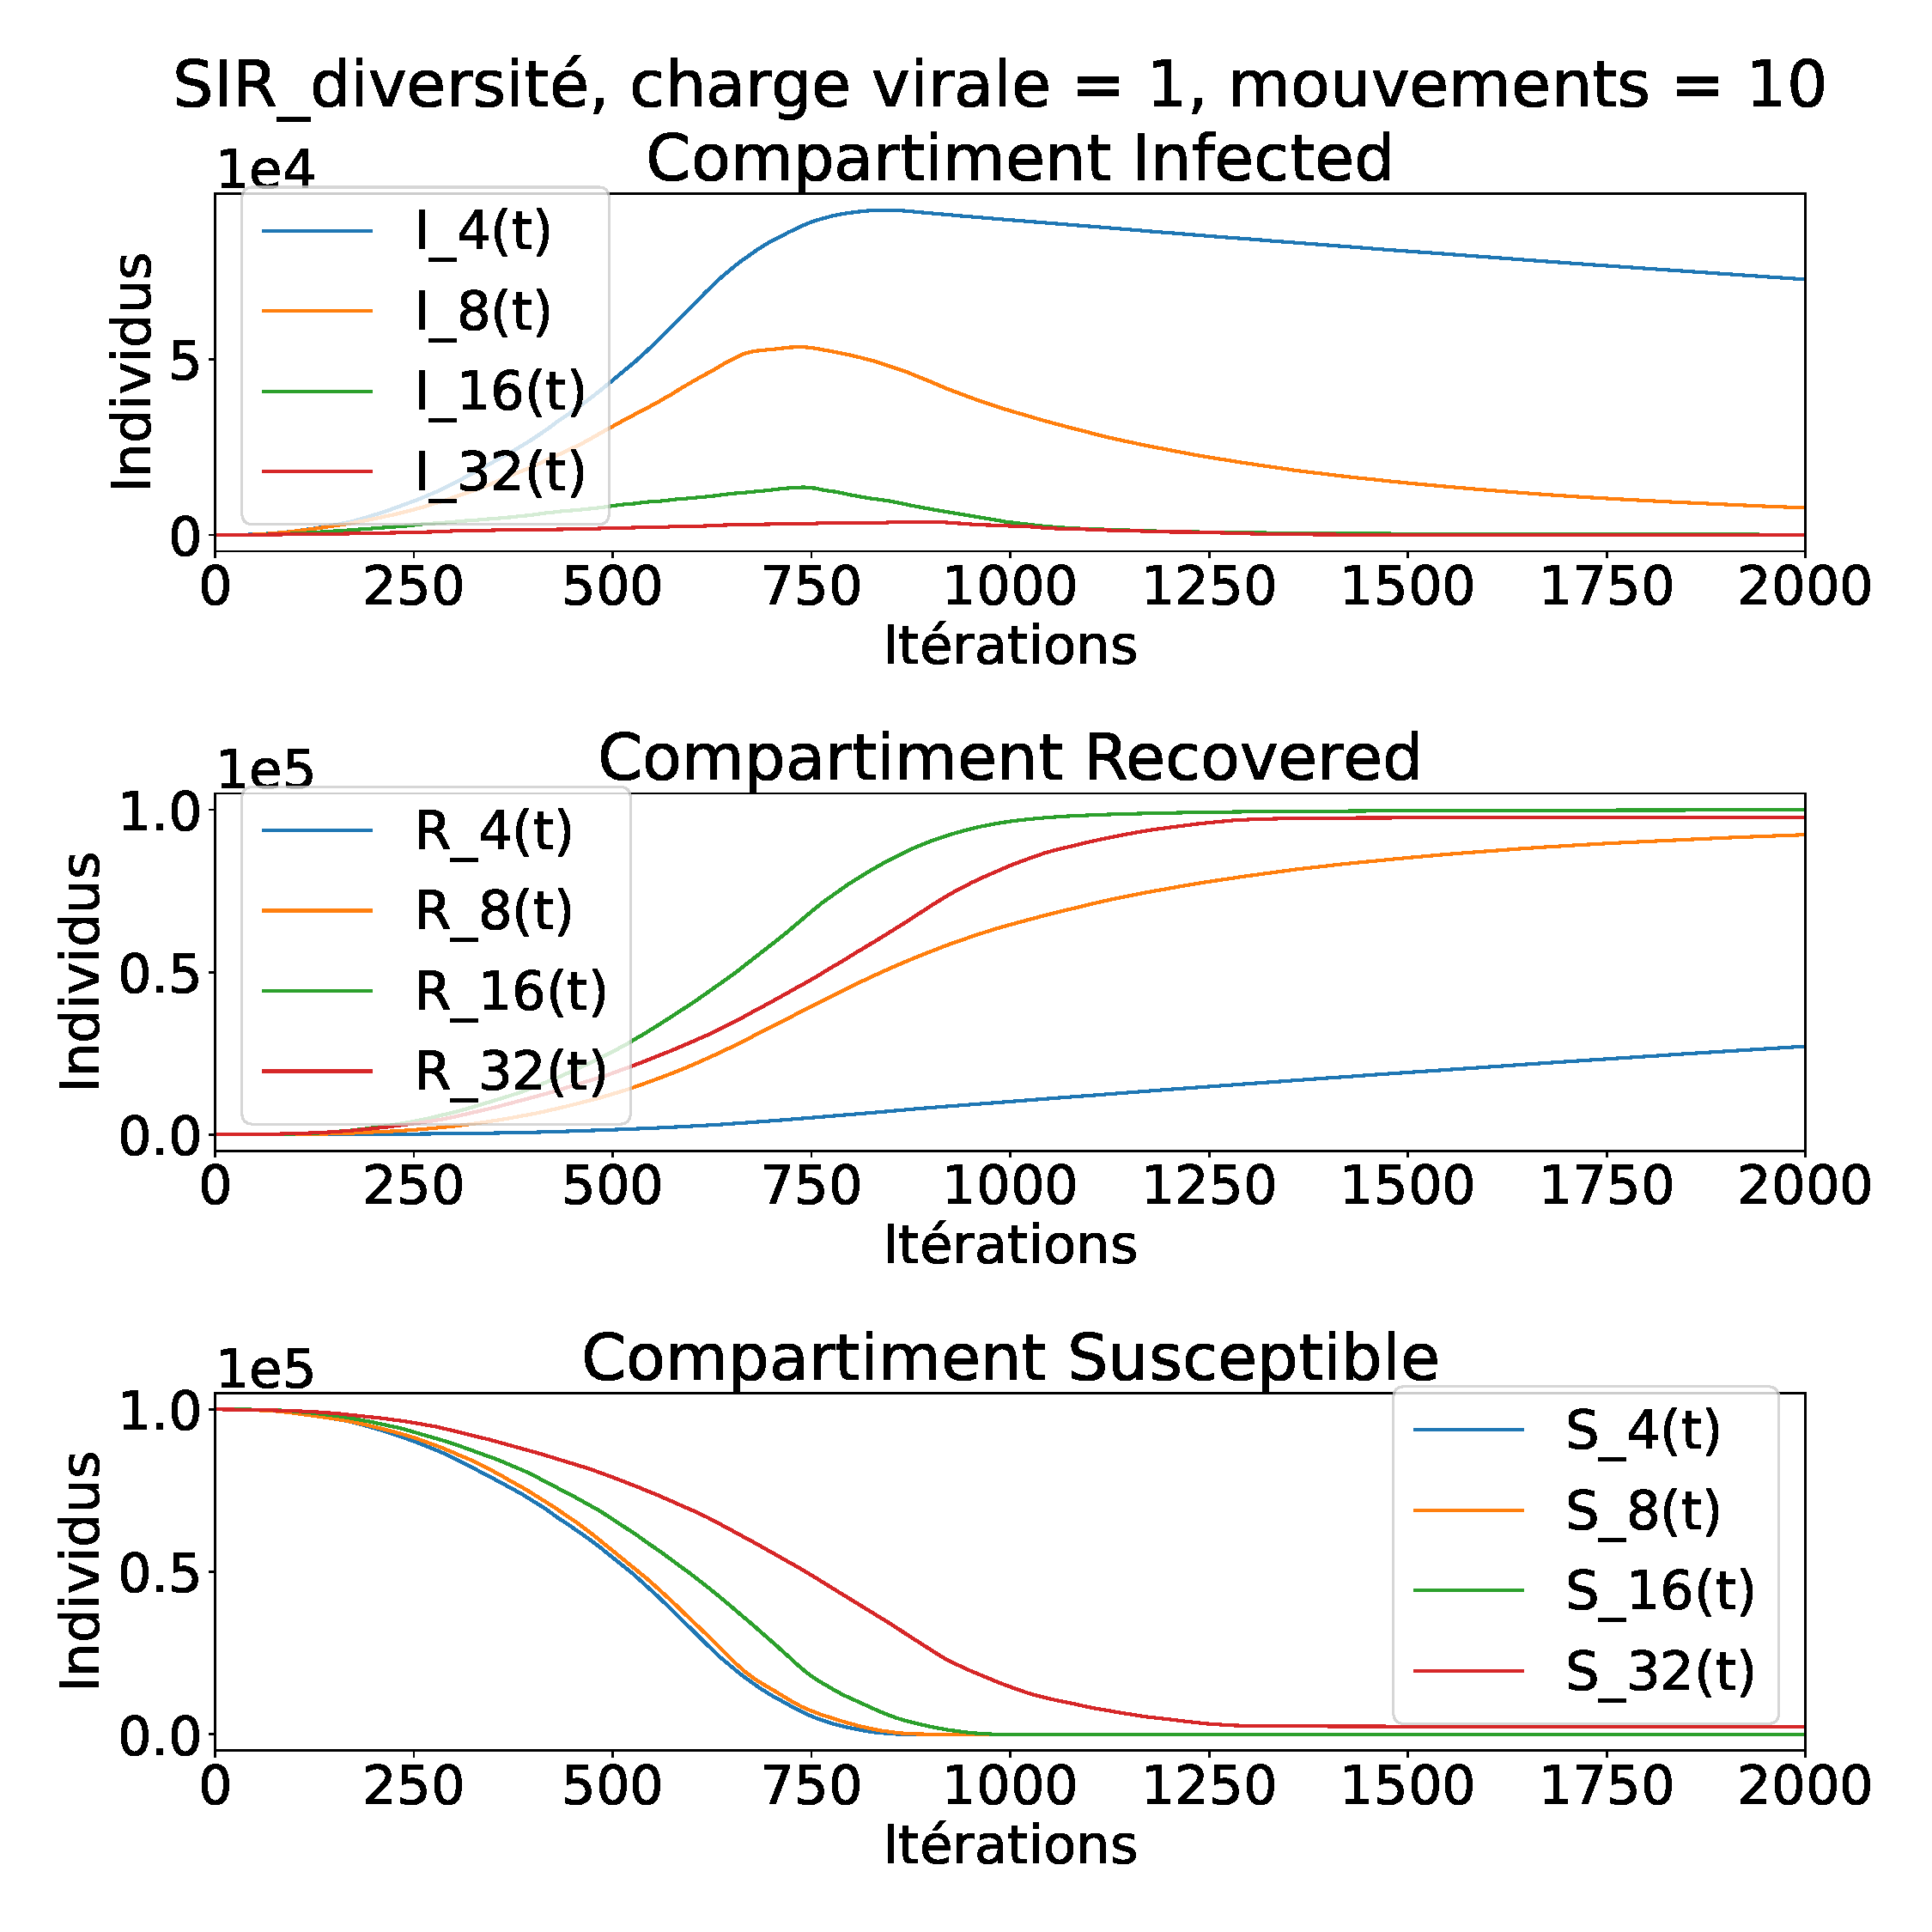
\includegraphics[width=.4\textwidth]{Images/SIR_diversite_1_10.pdf}
	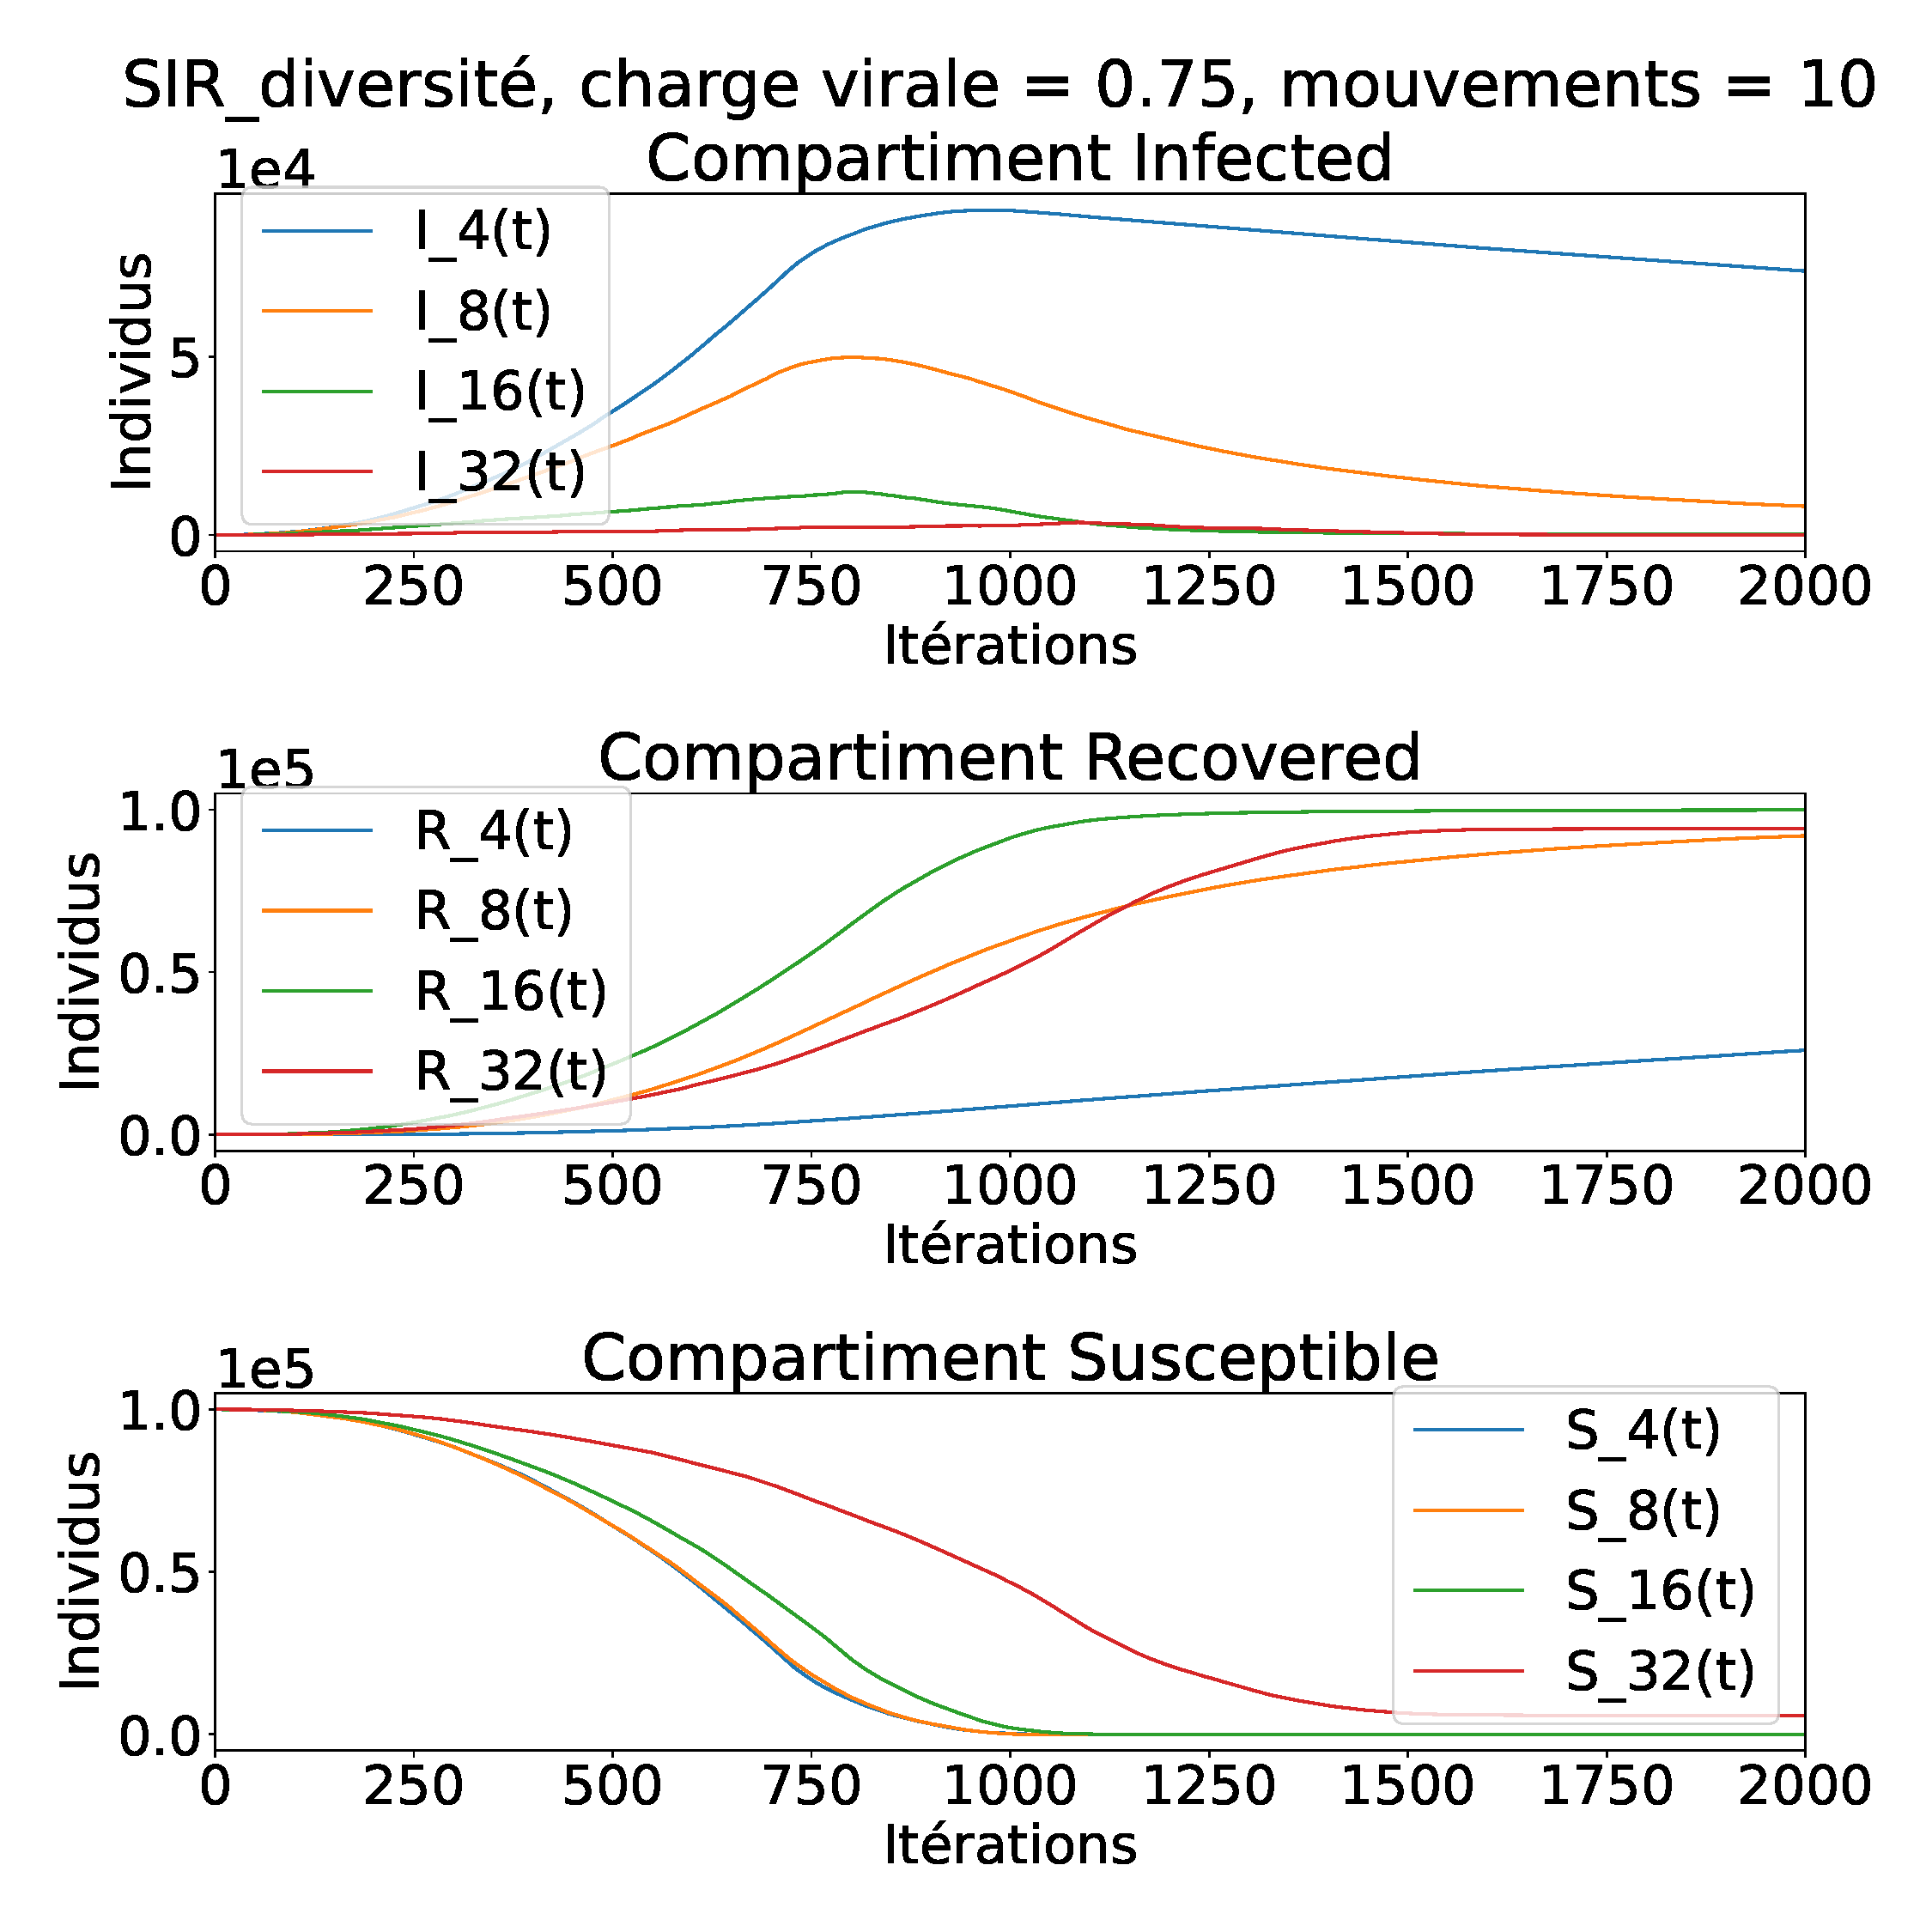
\includegraphics[width=.4\textwidth]{Images/SIR_diversite_075_10.pdf}
	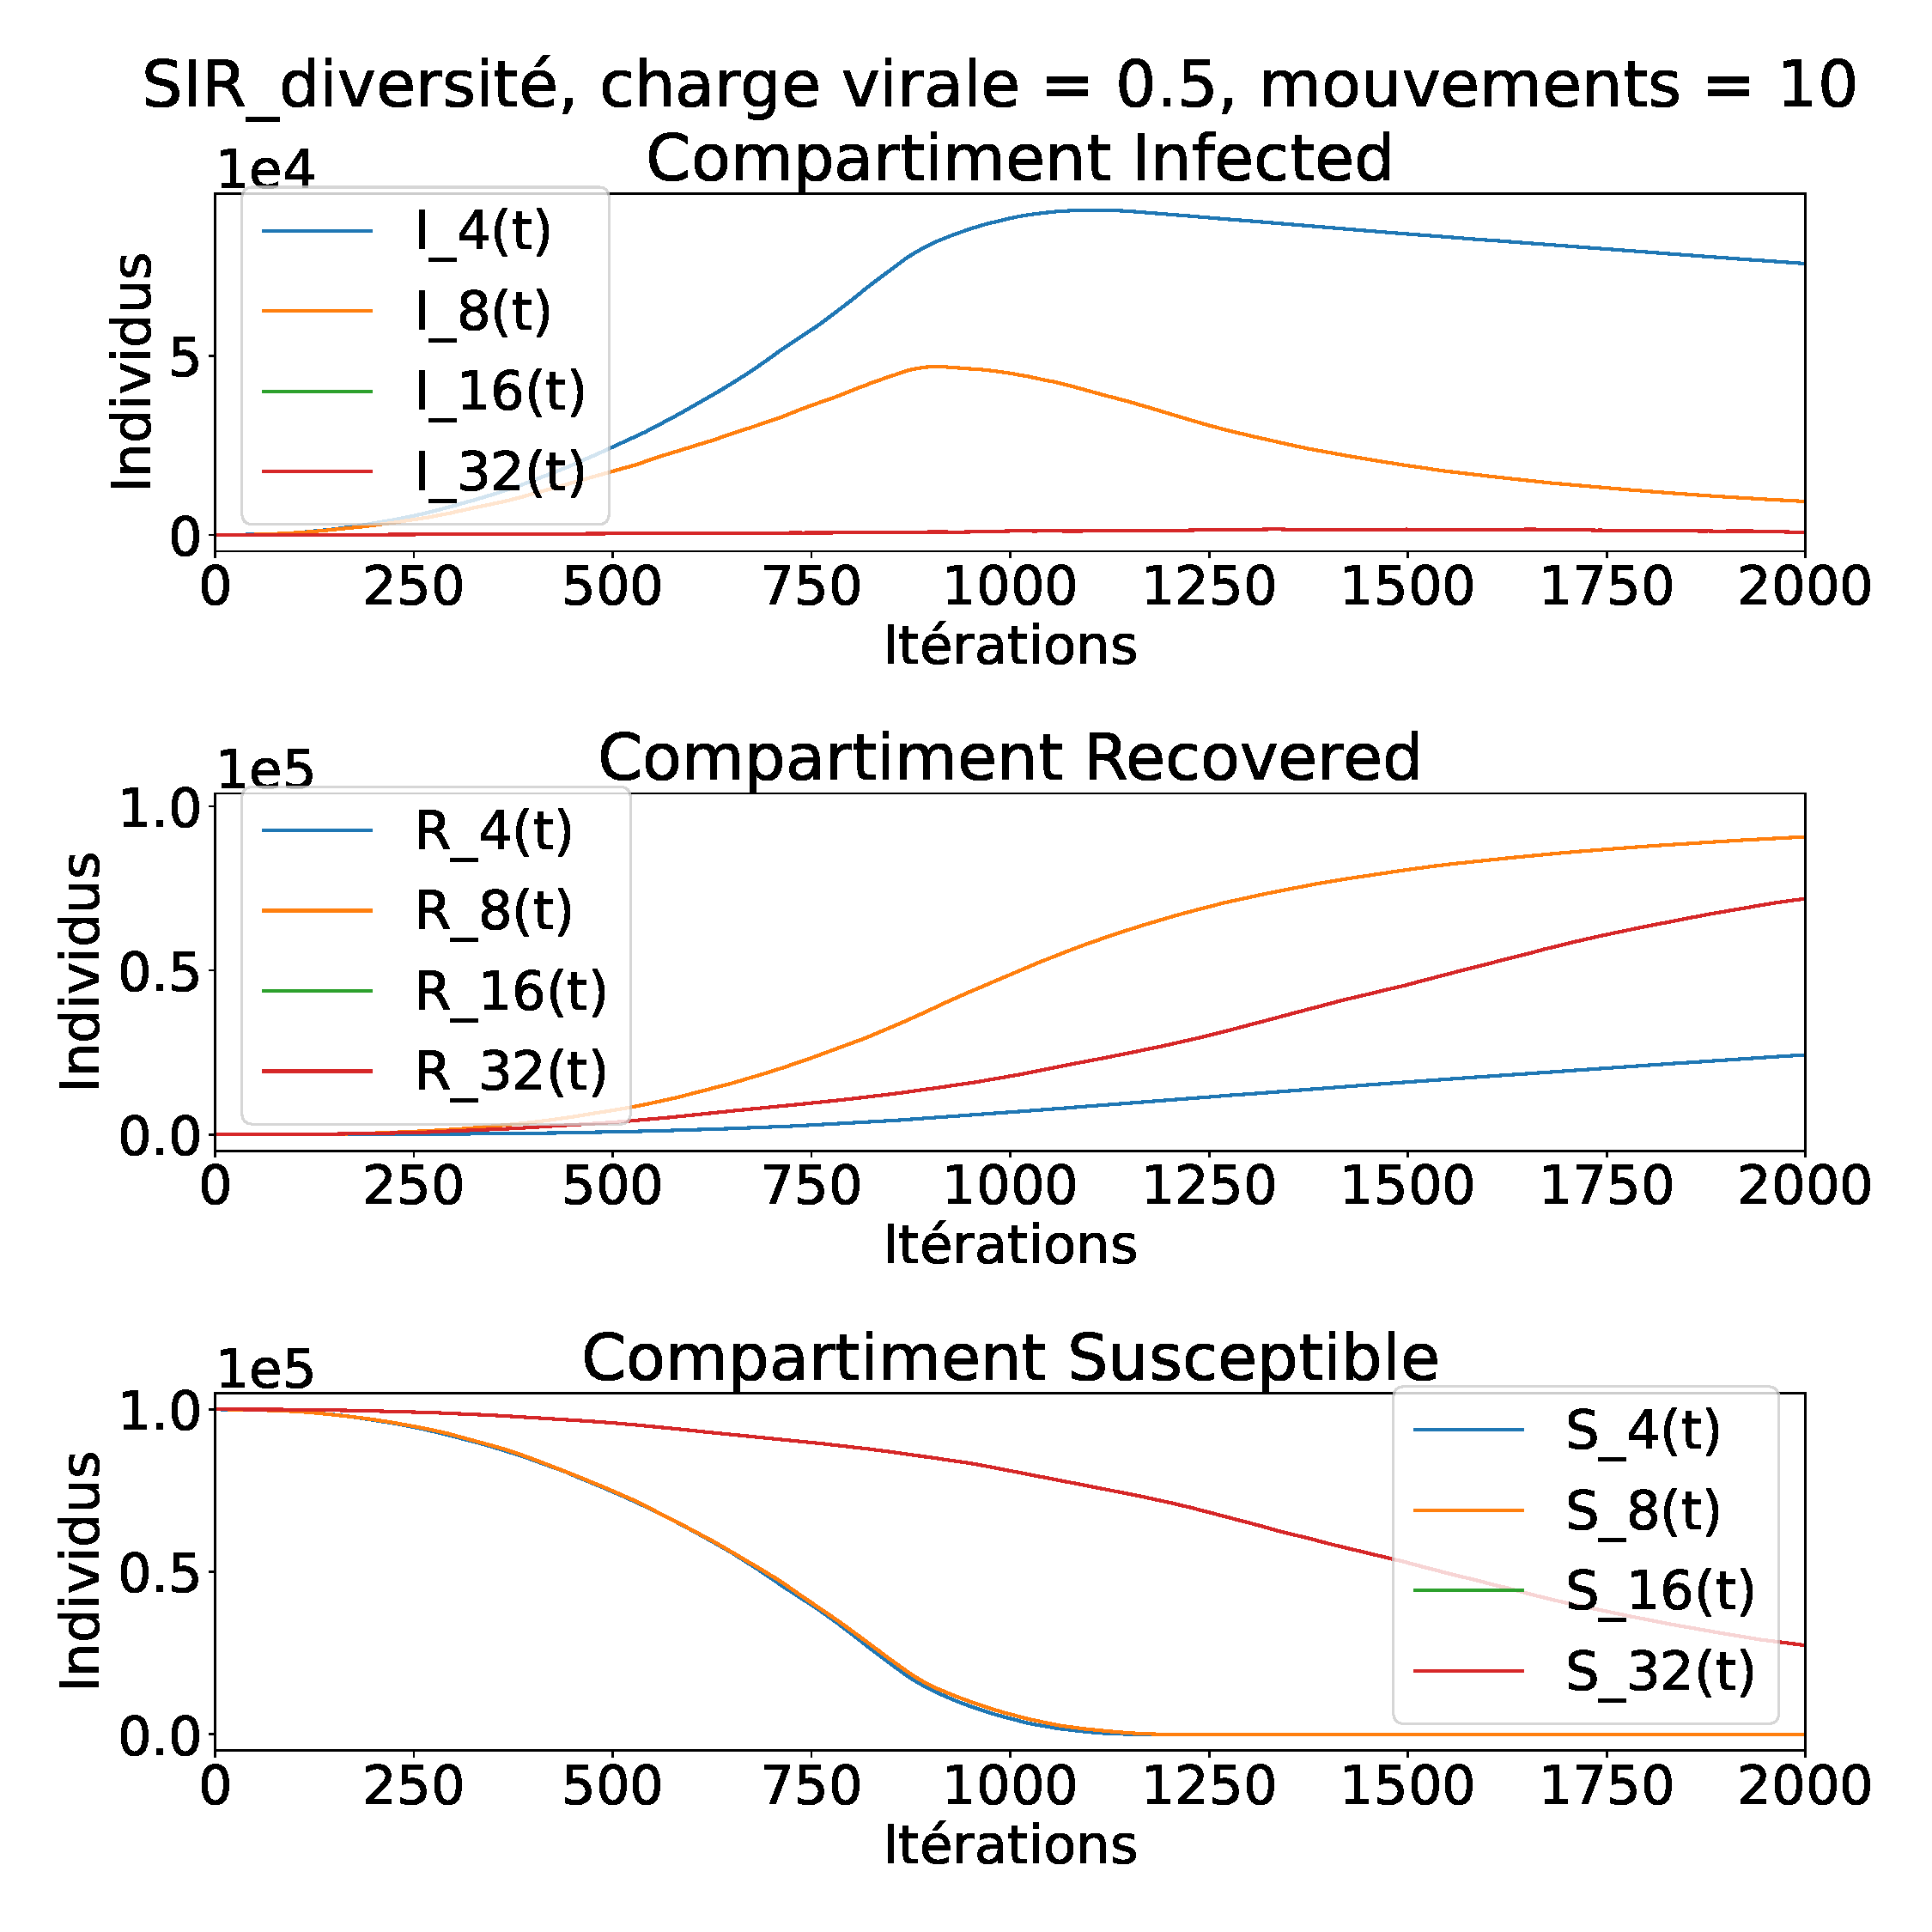
\includegraphics[width=.4\textwidth]{Images/SIR_diversite_05_10.pdf}
	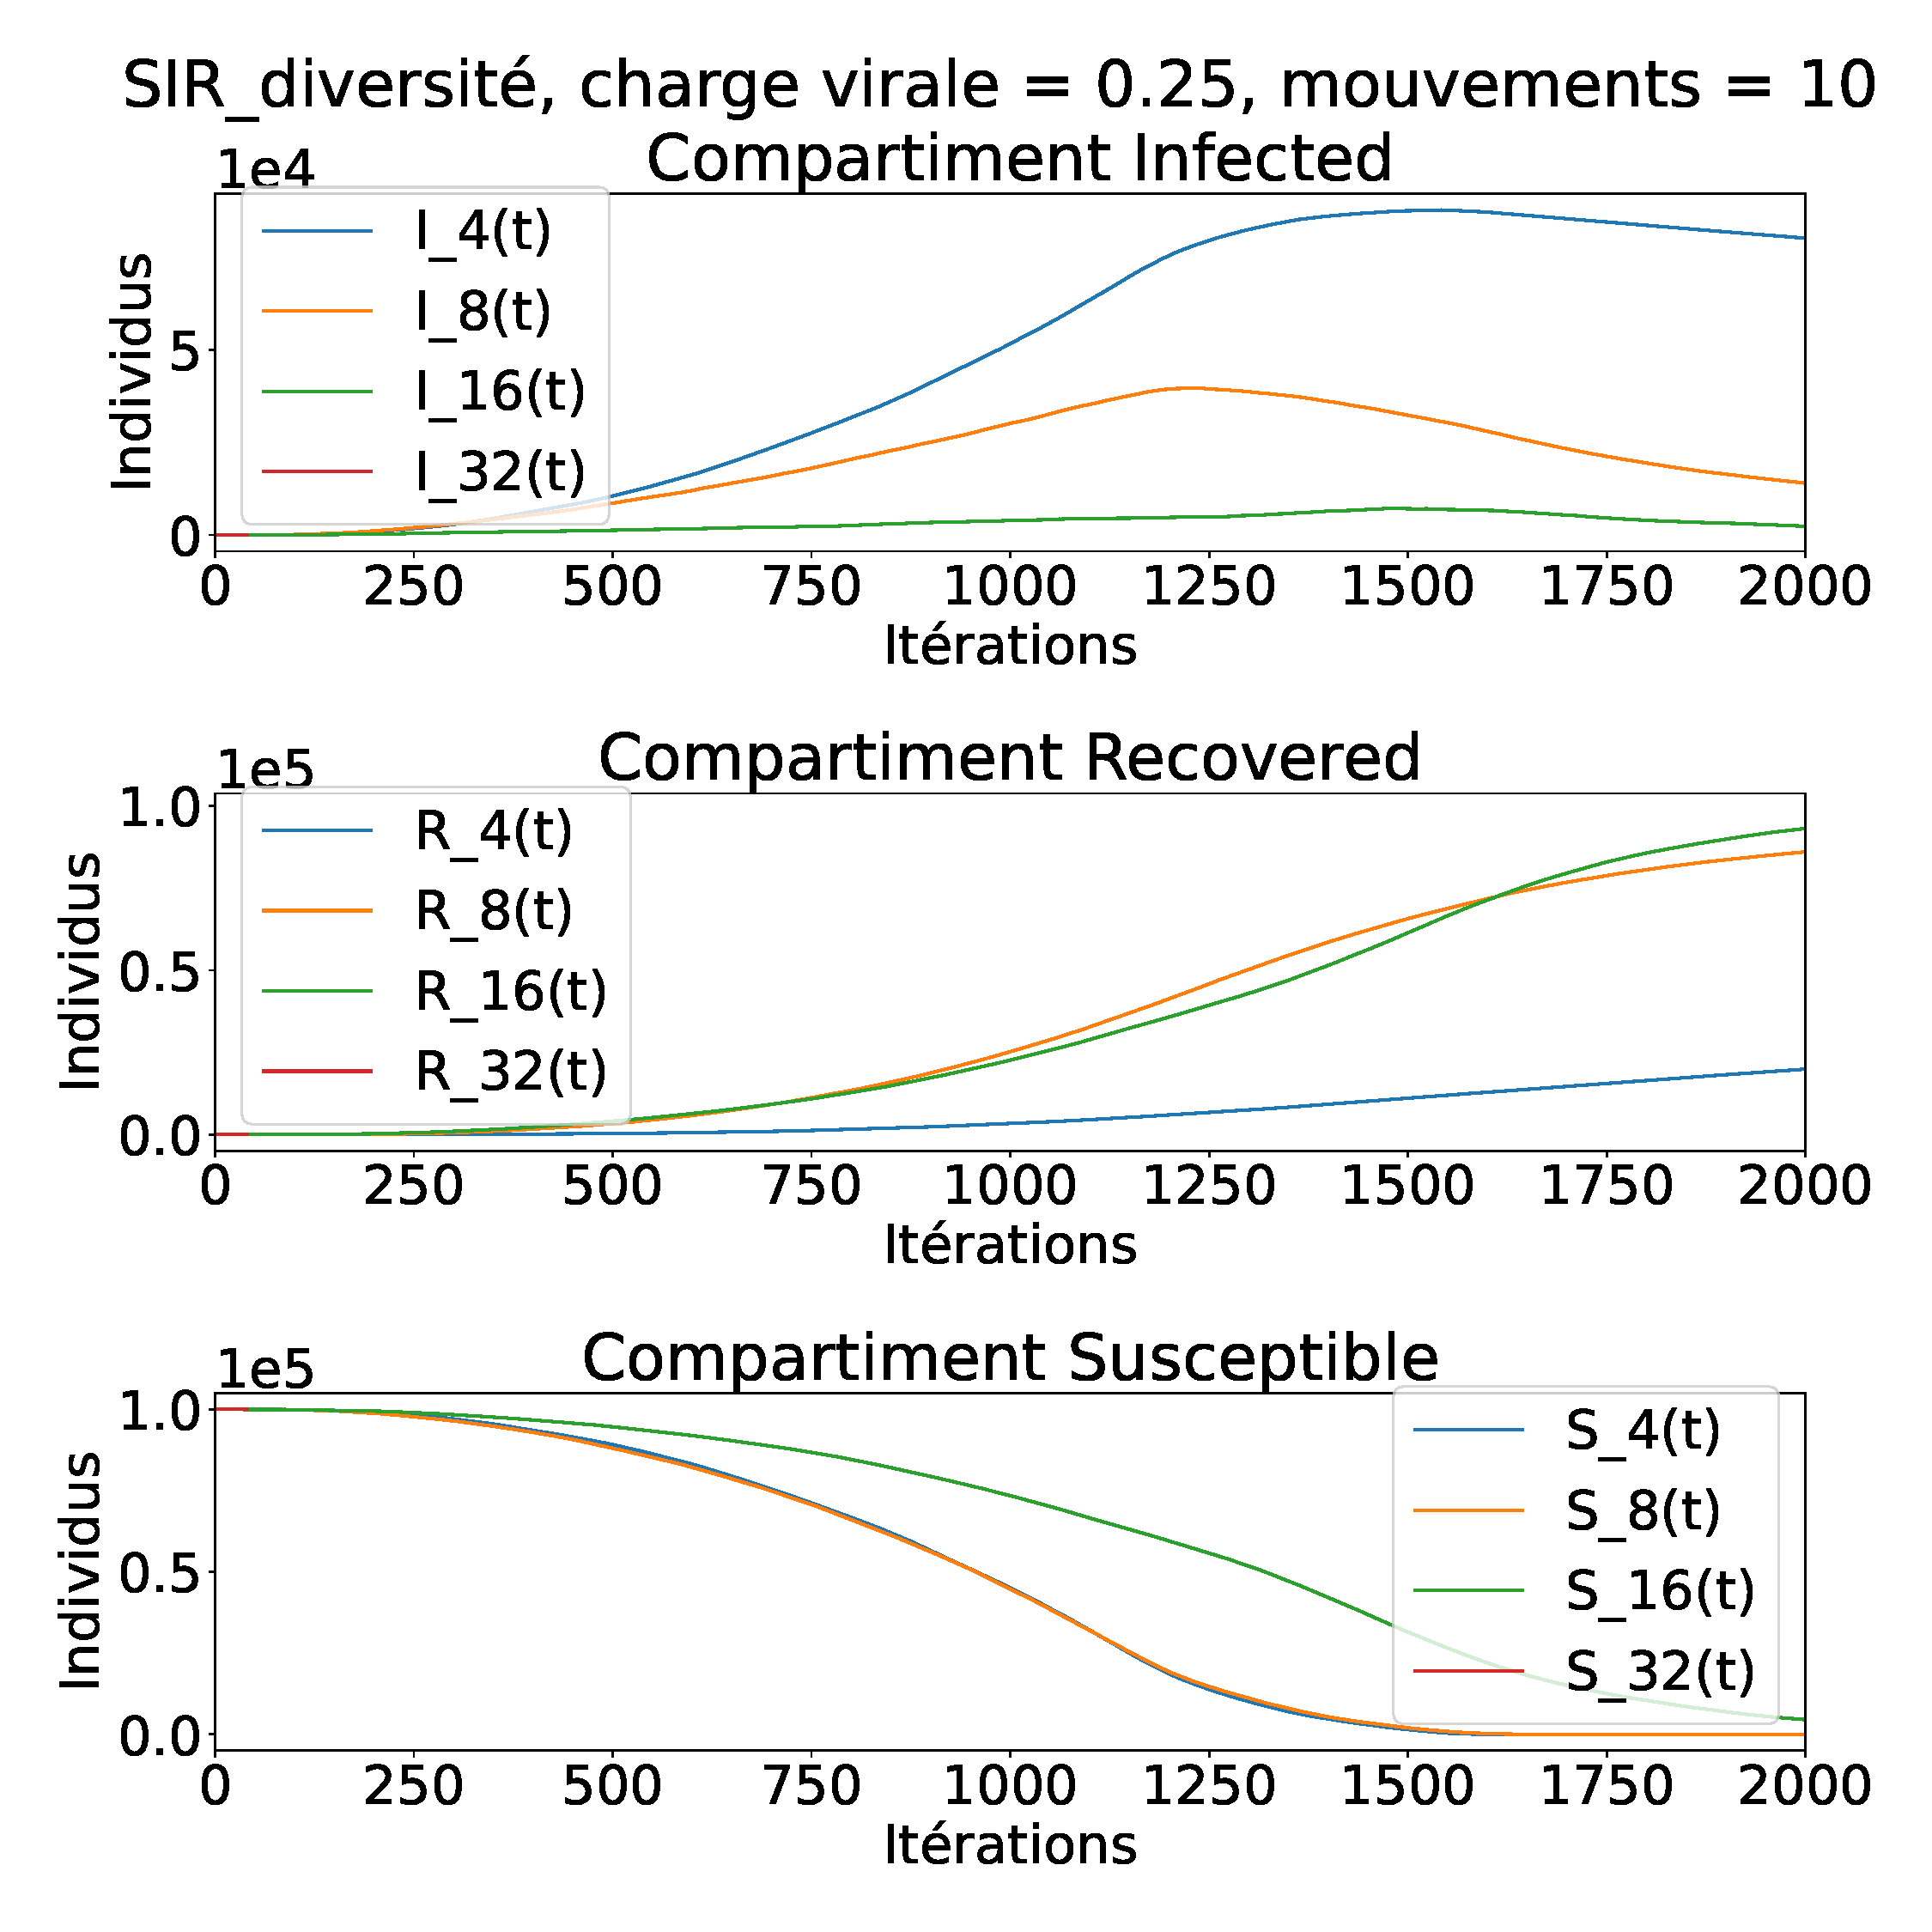
\includegraphics[width=.4\textwidth]{Images/SIR_diversite_025_10.pdf}
	\caption{Comparaison 10 mouvements}
\end{figure}

\newpage

\begin{figure}[h]
	\centering
	\captionsetup{justification=centering}
	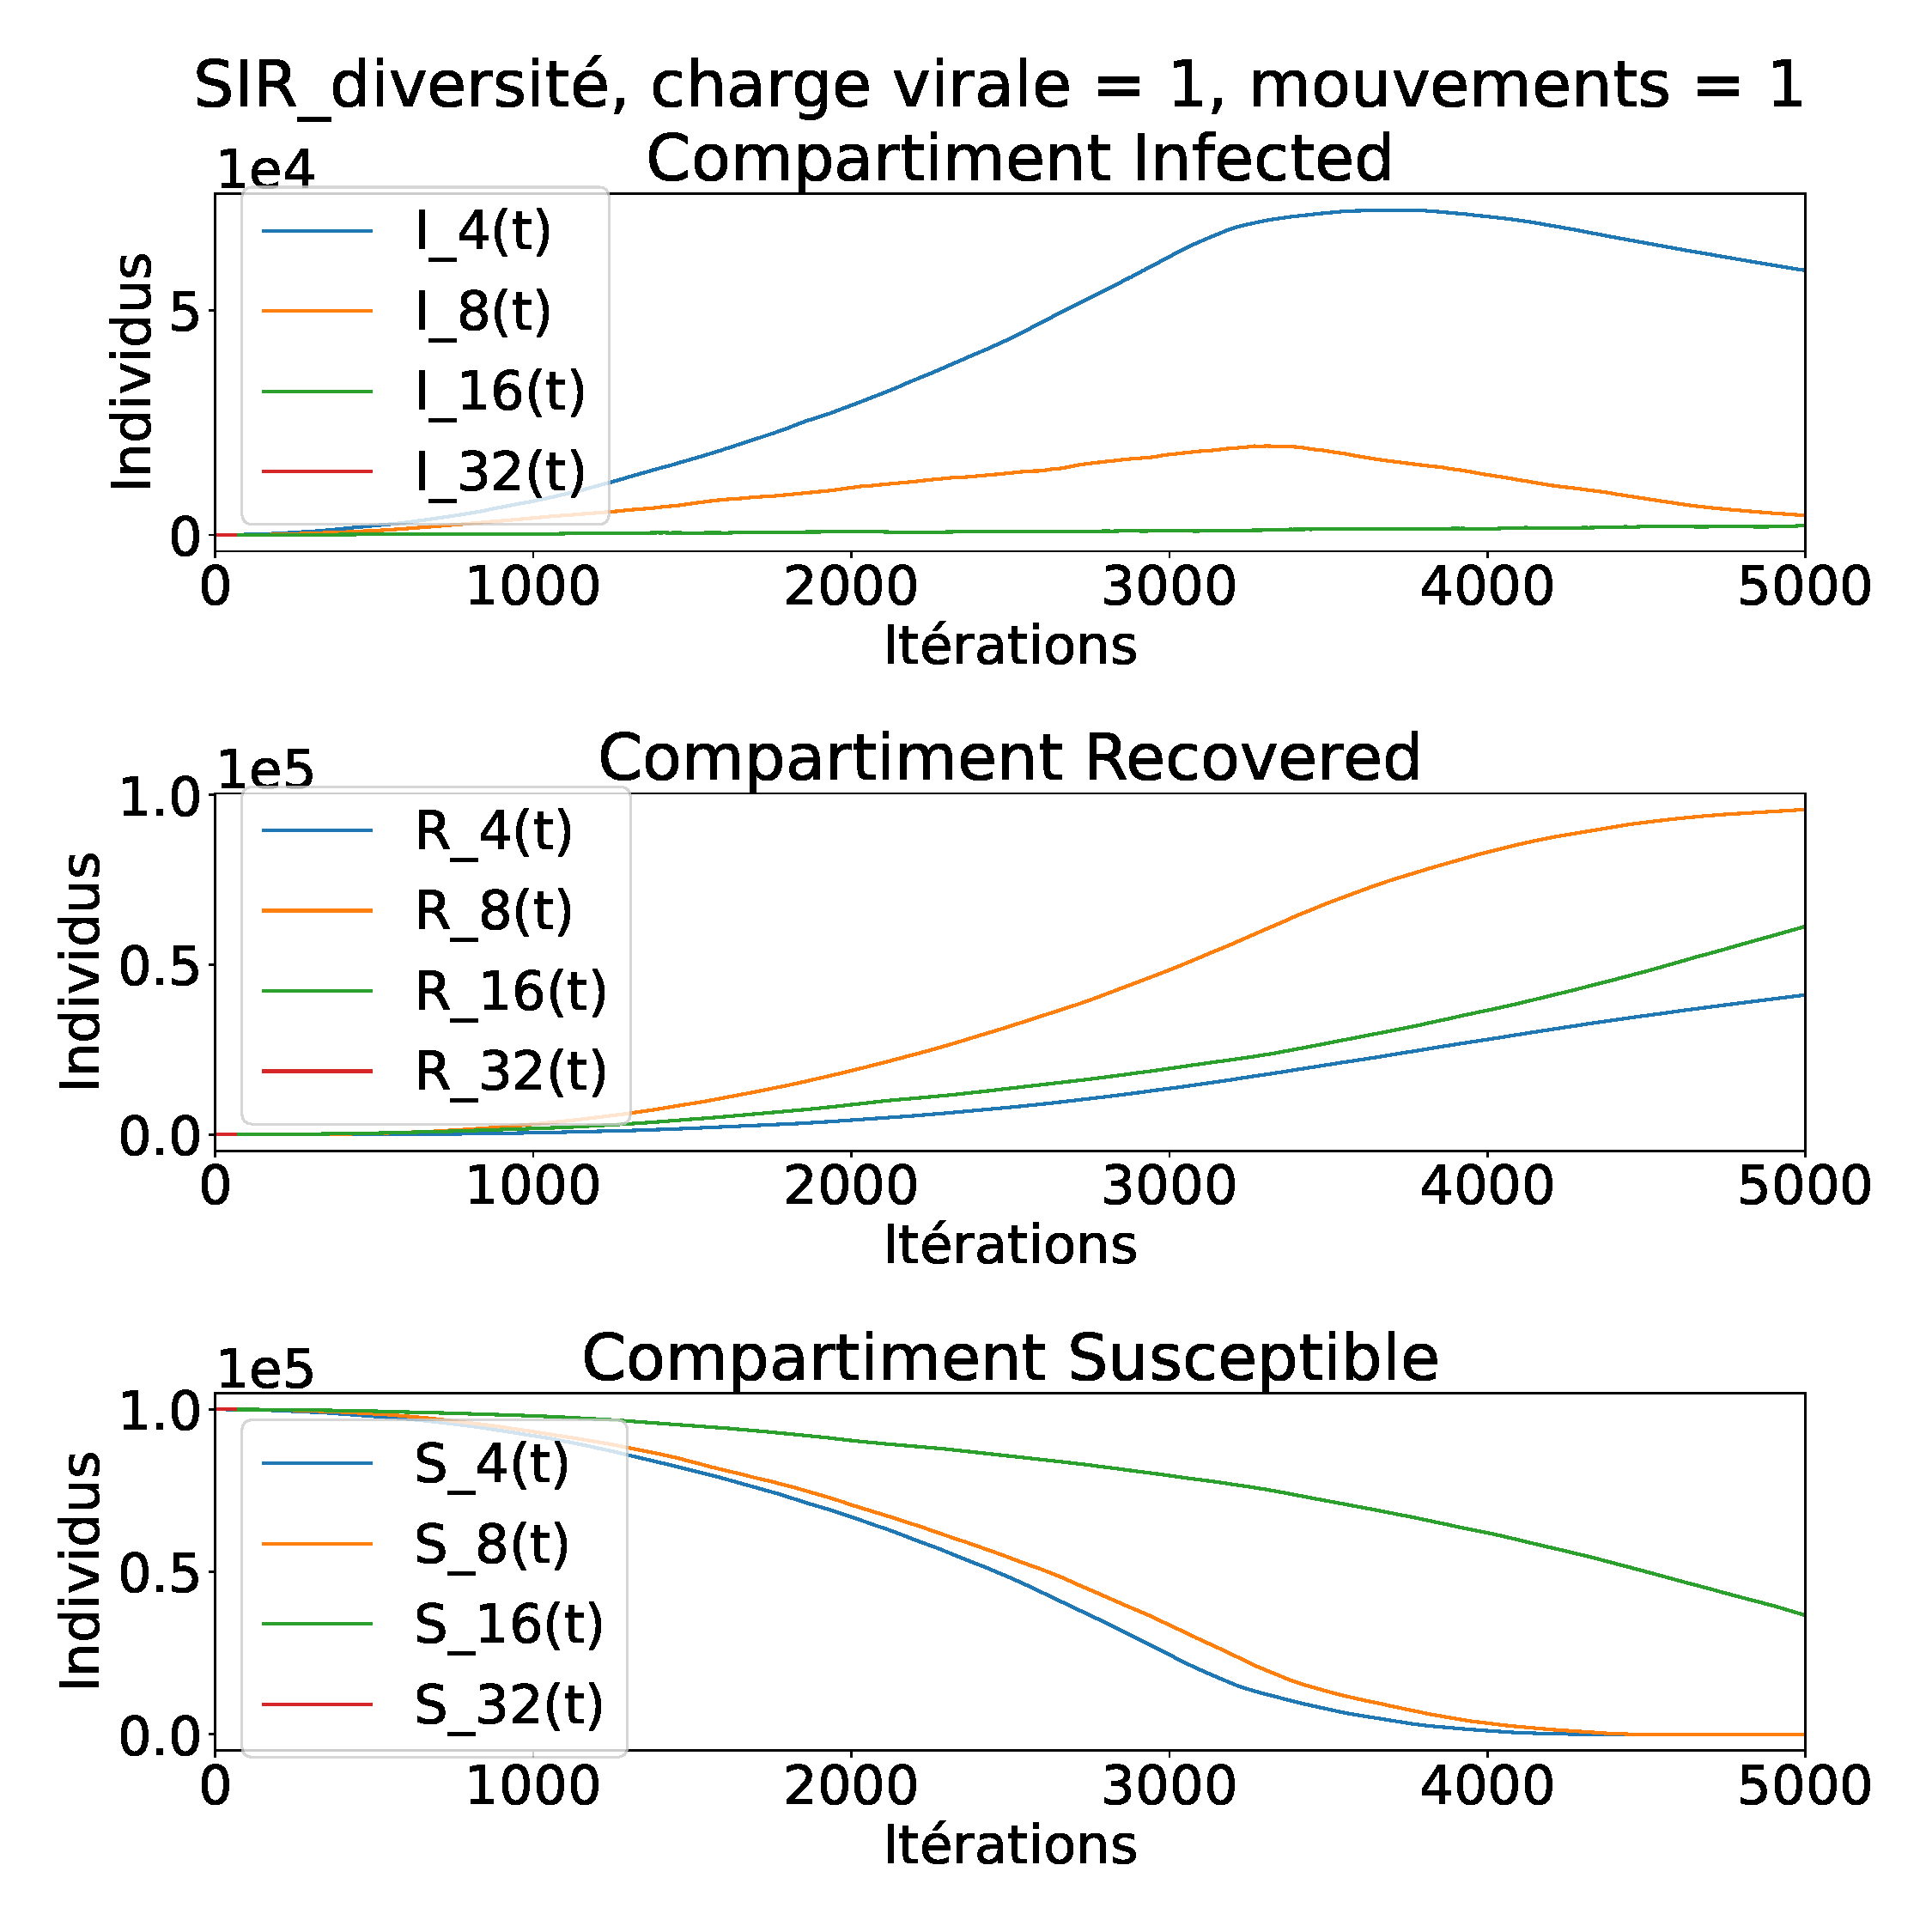
\includegraphics[width=.4\textwidth]{Images/SIR_diversite_1_1.pdf}
	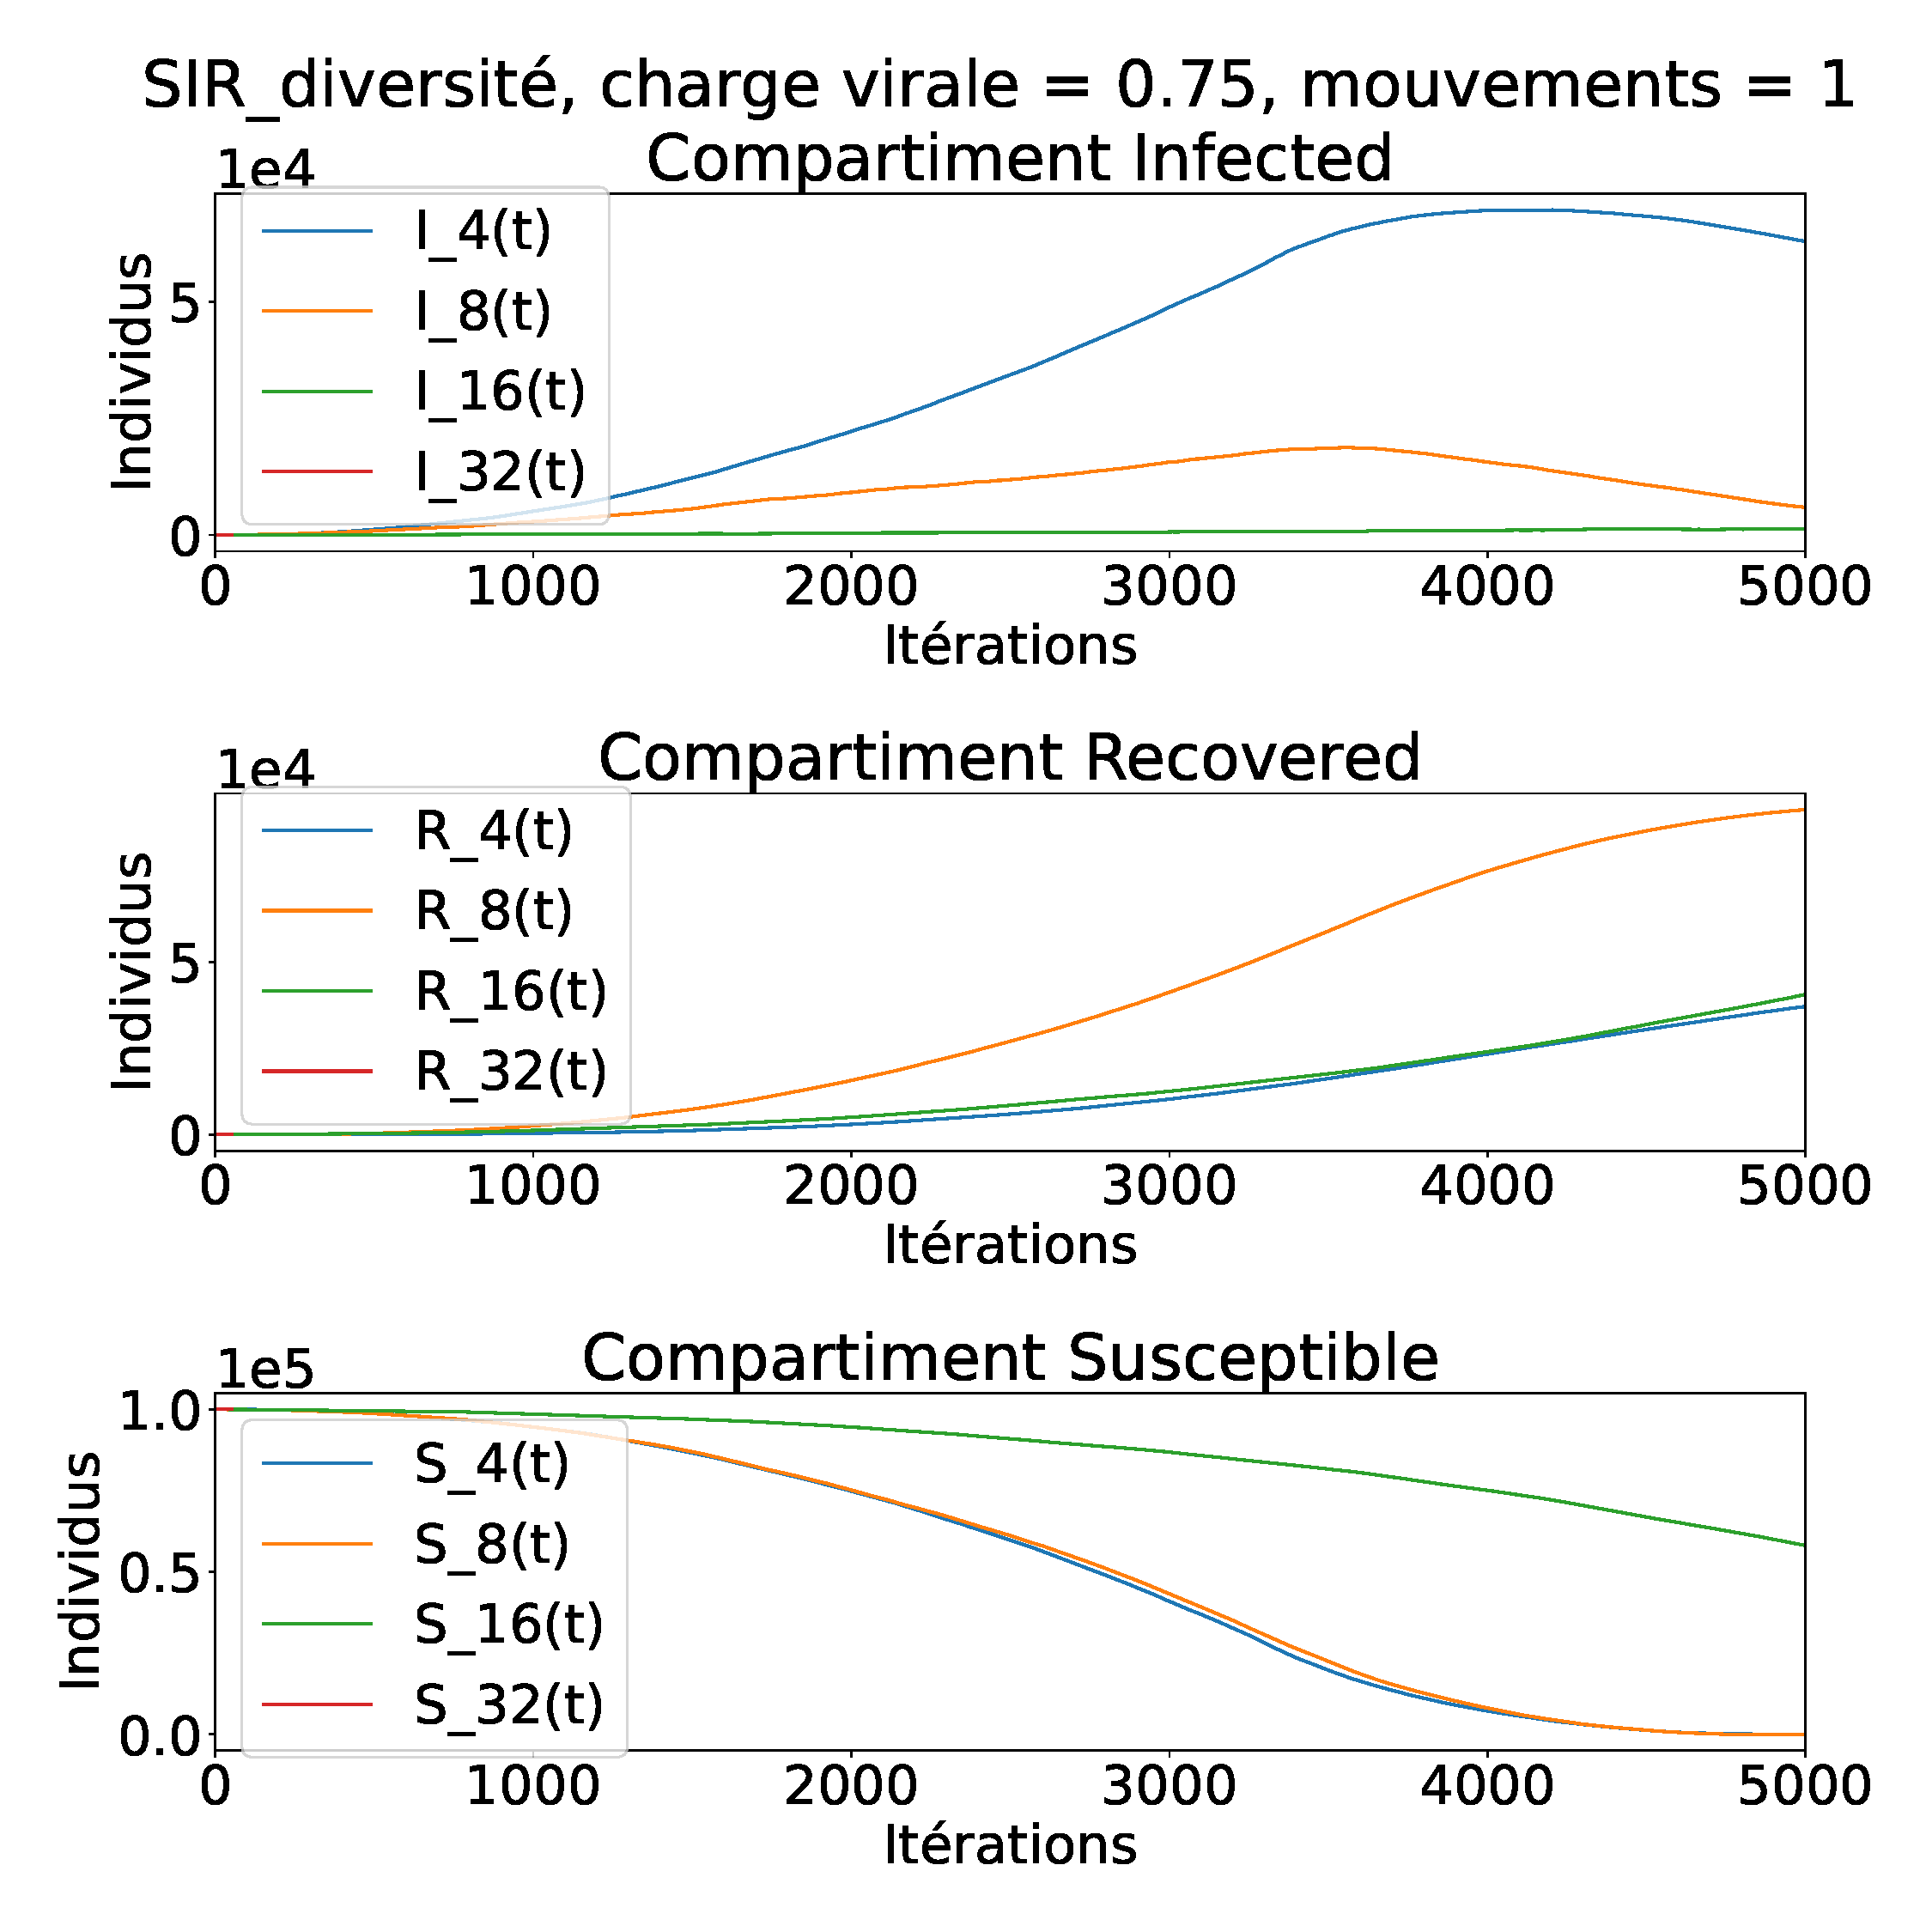
\includegraphics[width=.4\textwidth]{Images/SIR_diversite_075_1.pdf}
	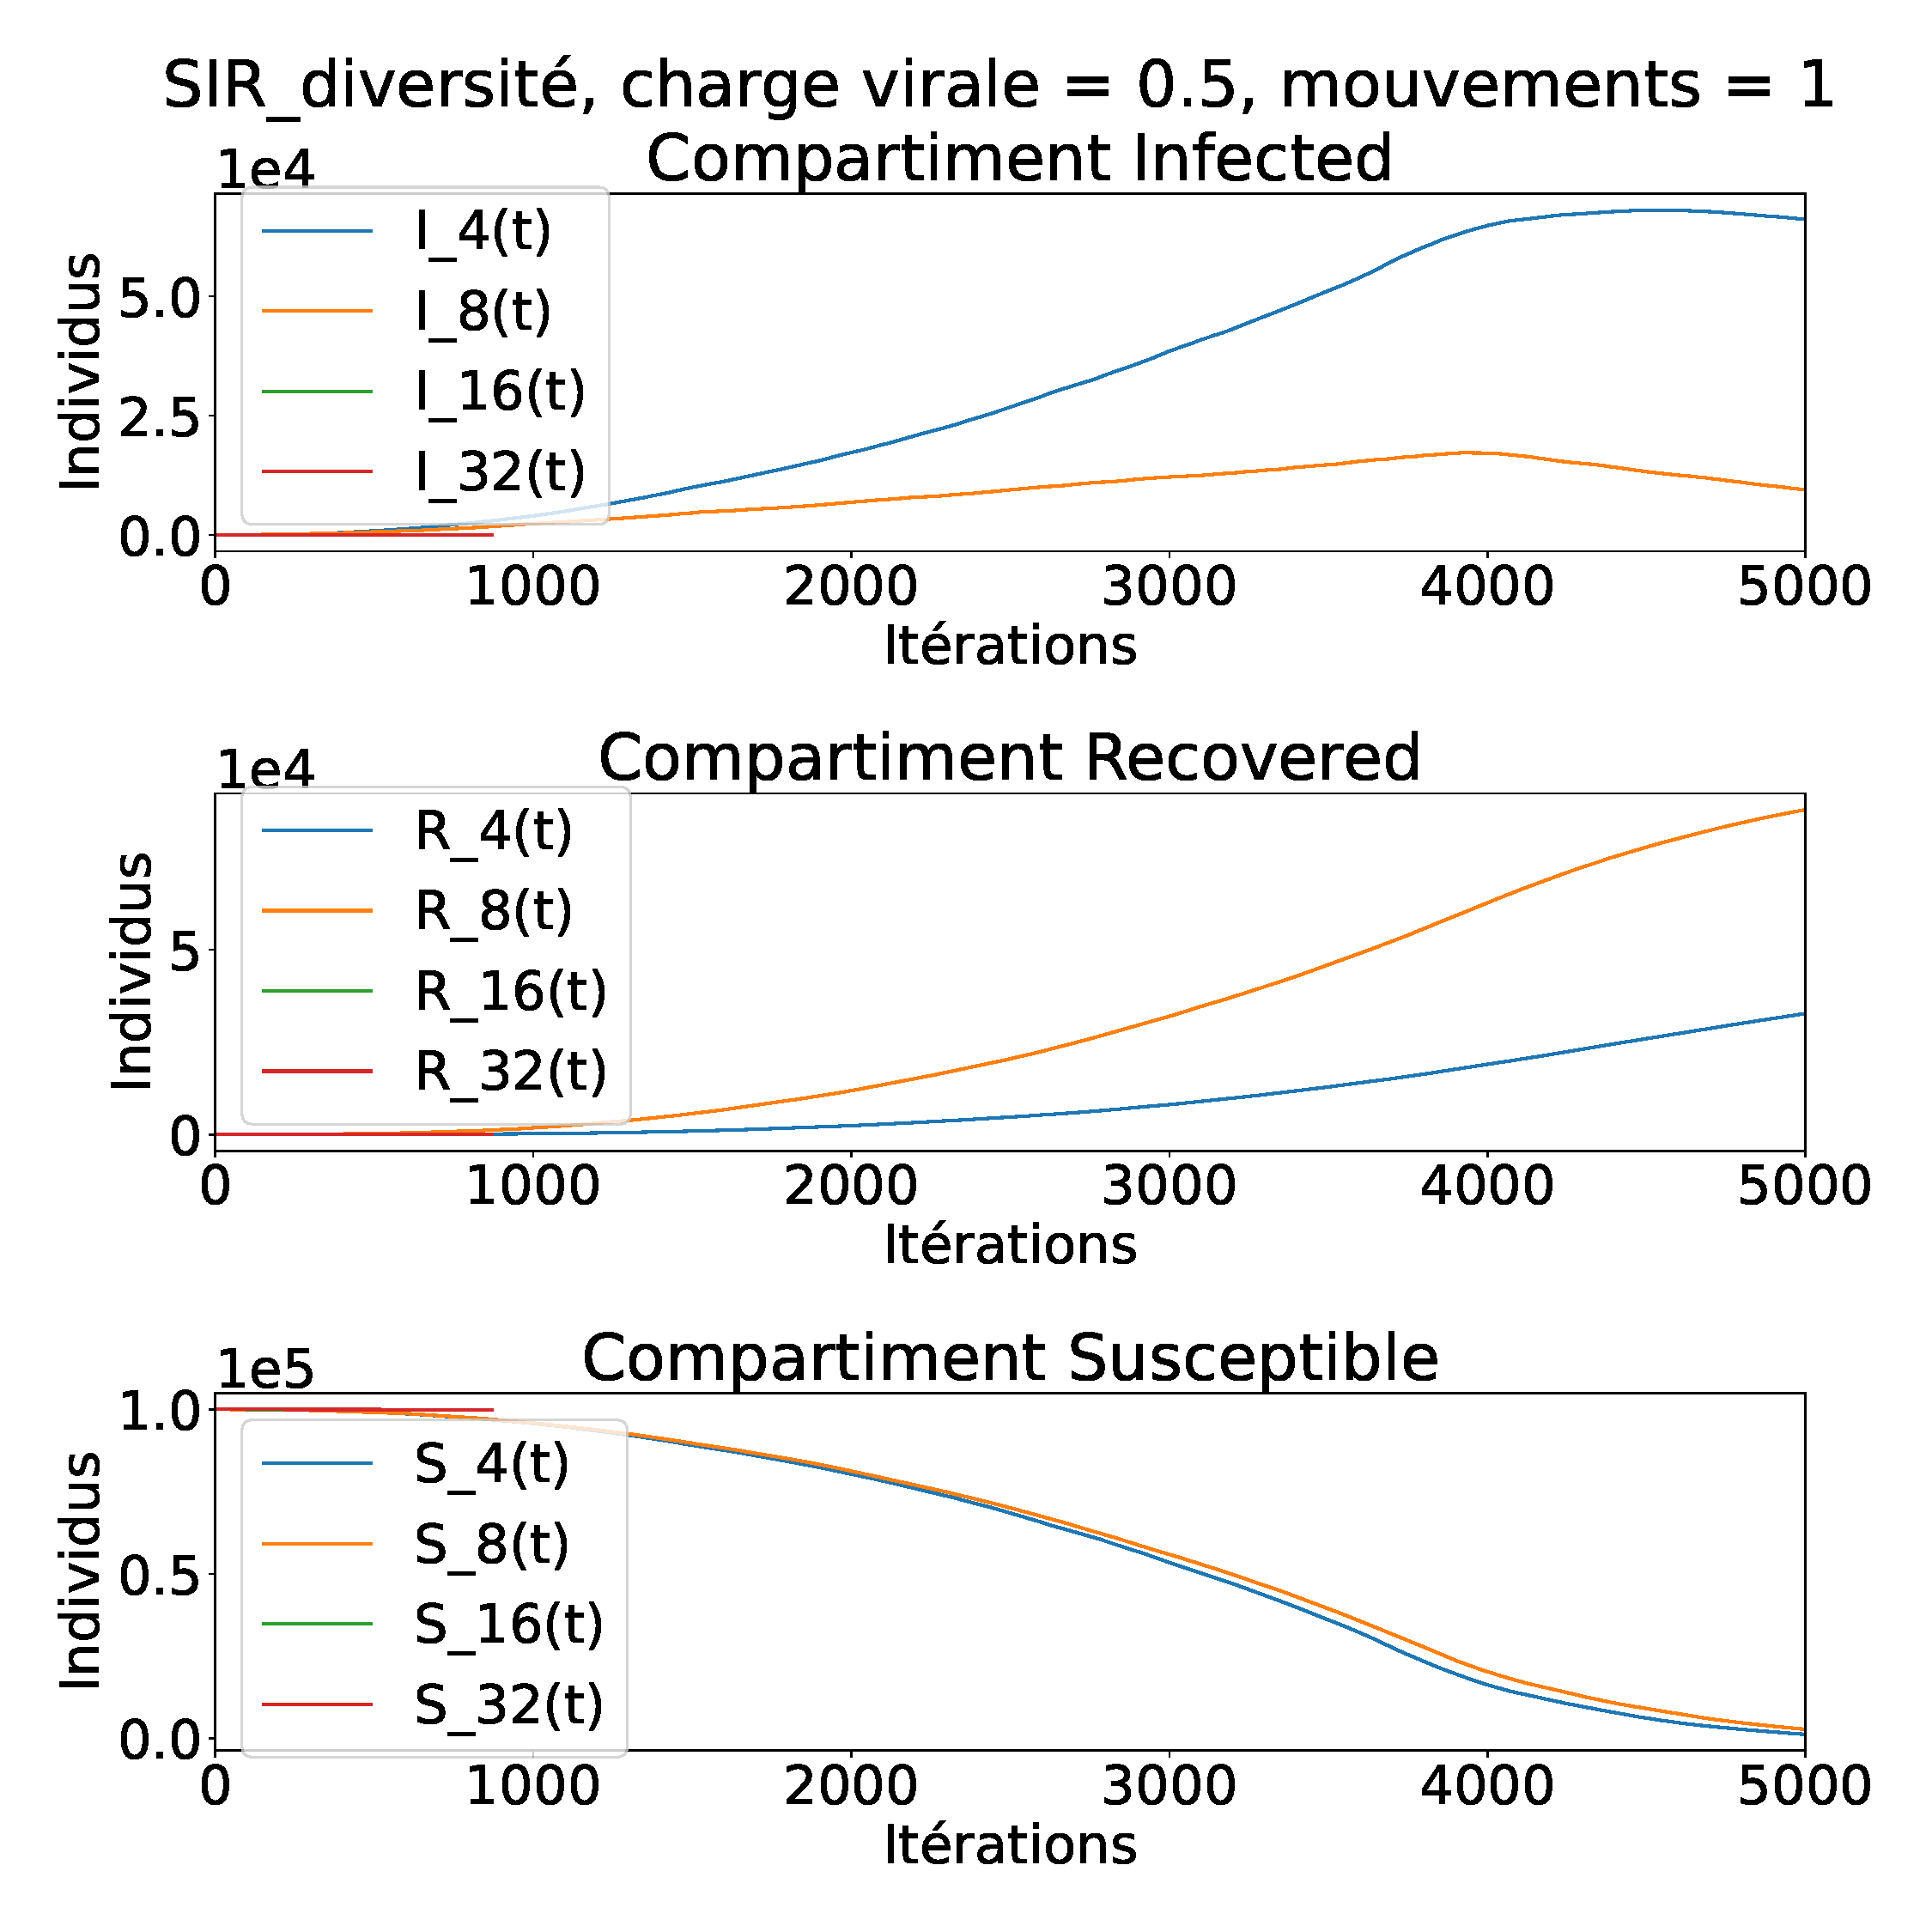
\includegraphics[width=.4\textwidth]{Images/SIR_diversite_05_1.pdf}
	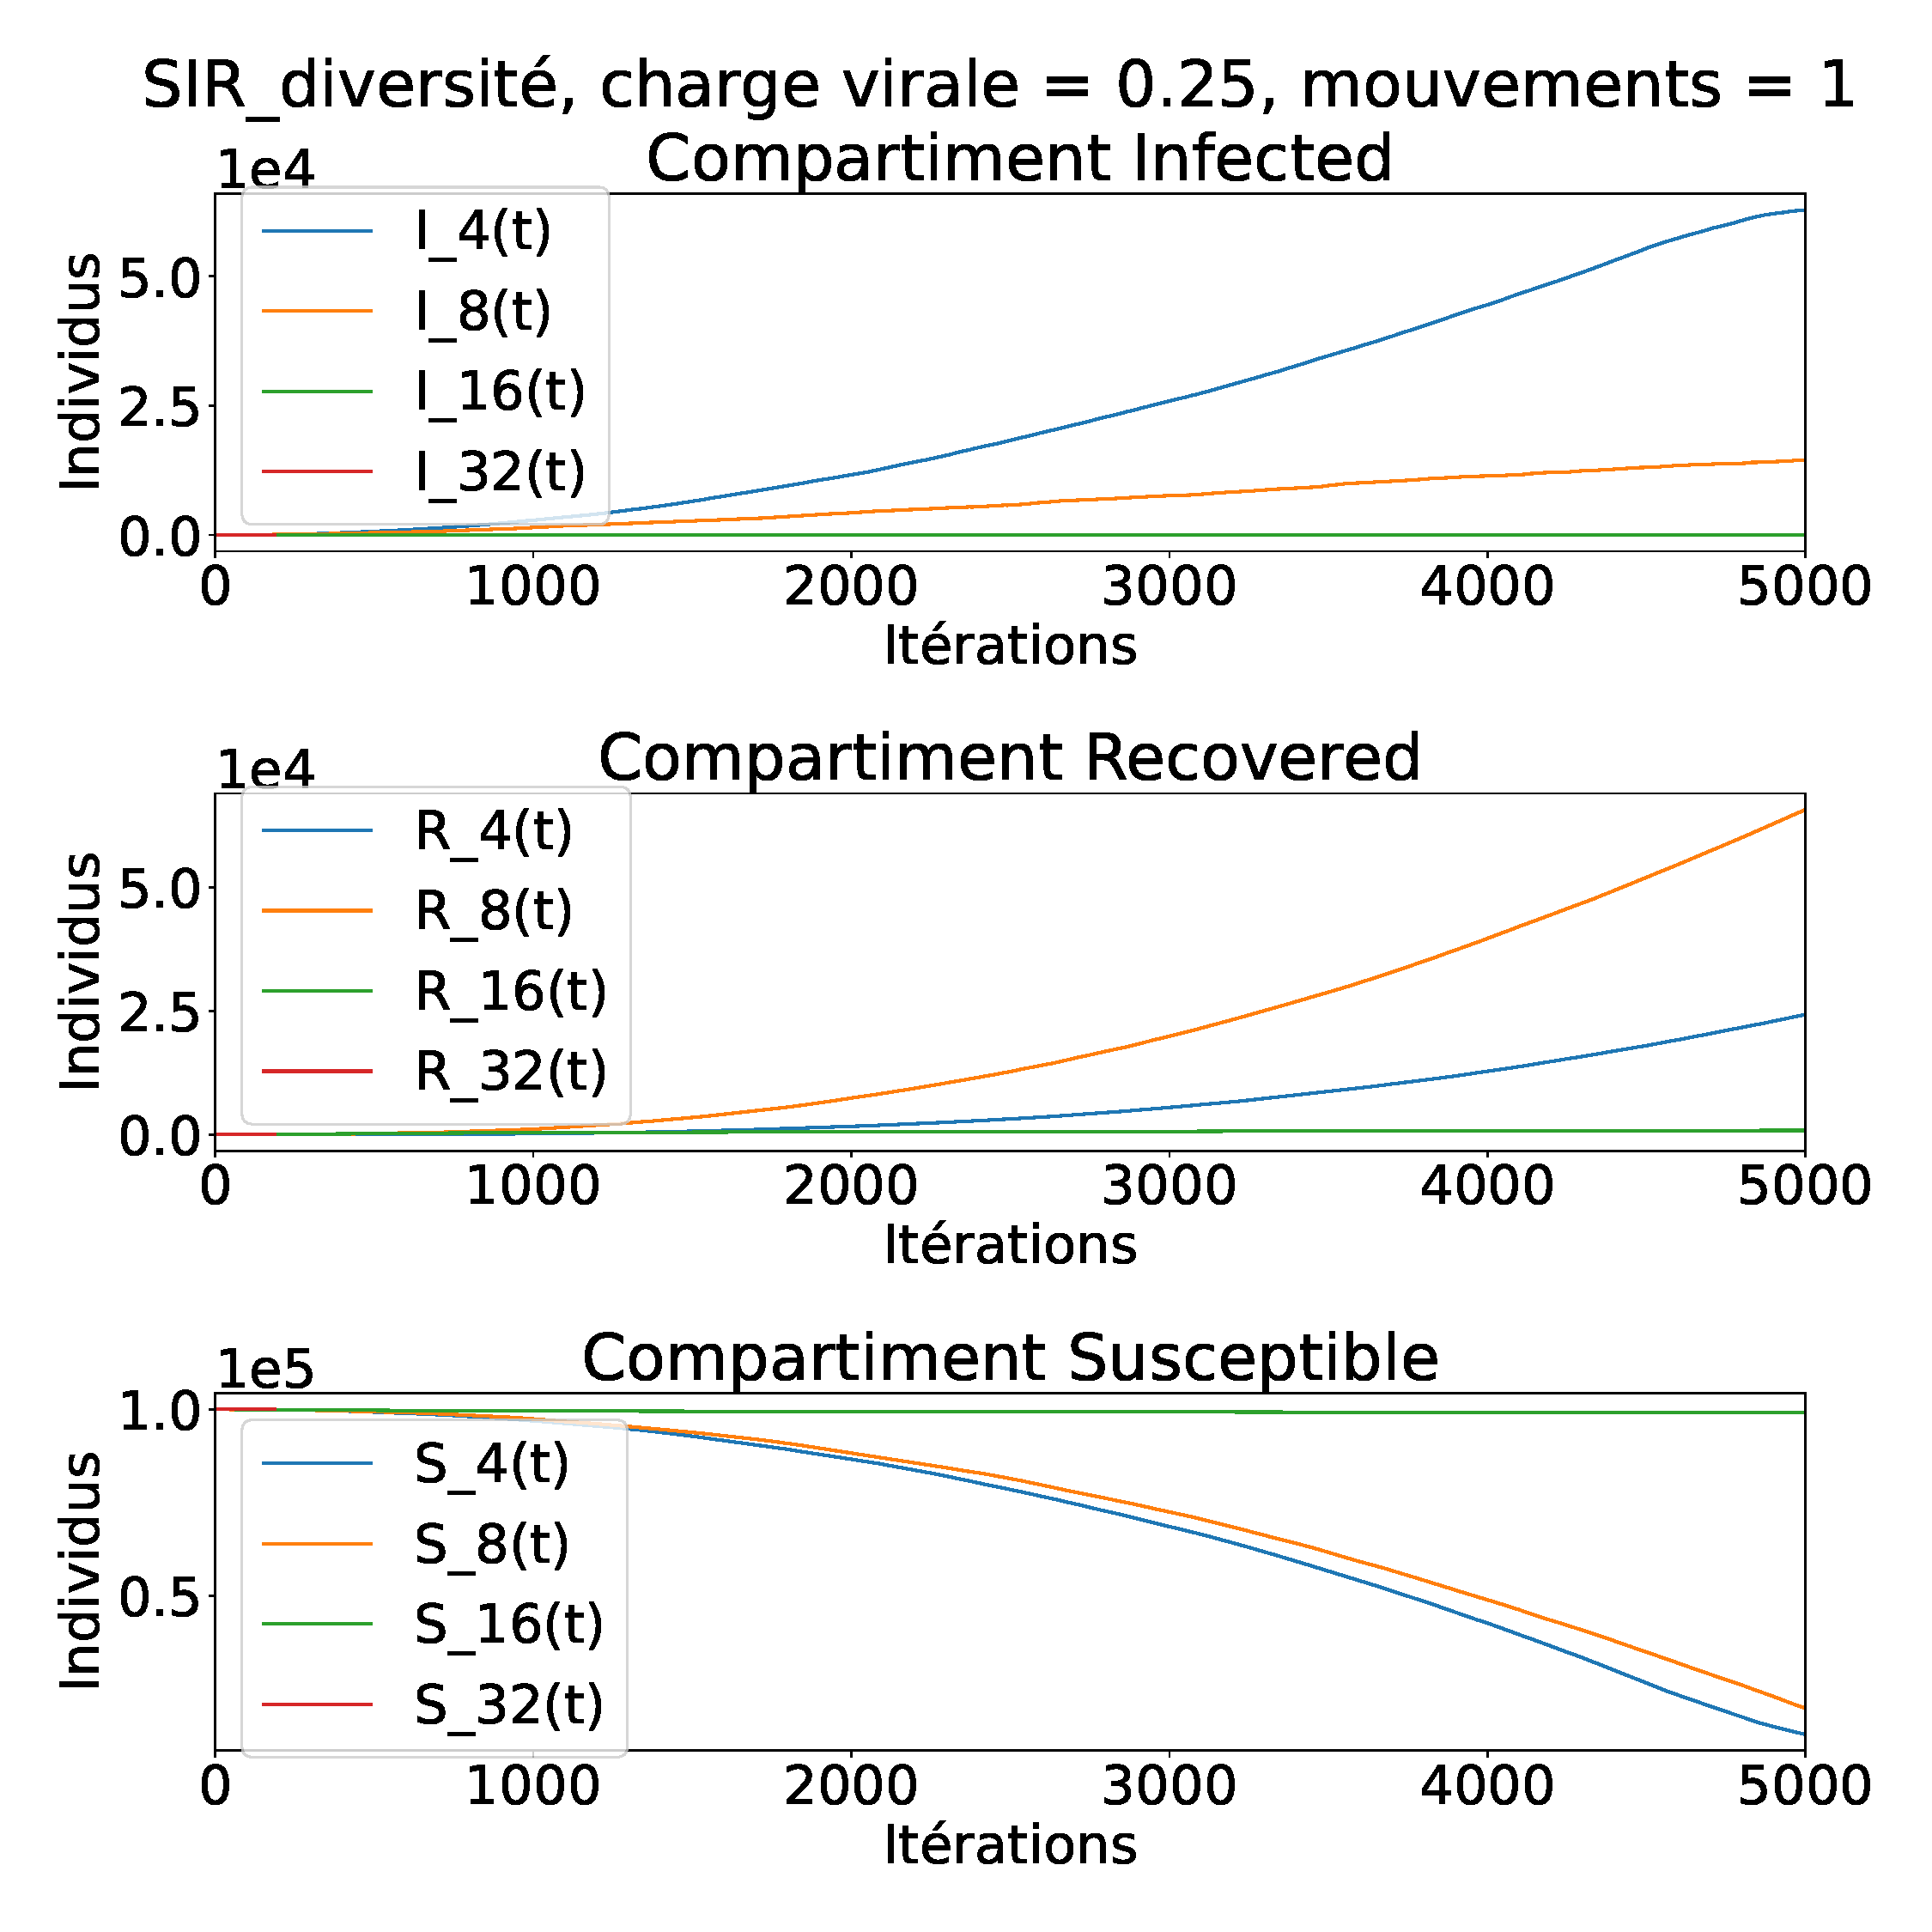
\includegraphics[width=.4\textwidth]{Images/SIR_diversite_025_1.pdf}
	\caption{Comparaison 1 mouvements}
\end{figure}

\section{Analyses}

